\lhead{\begin{tikzpicture}[remember picture, overlay]
    \node [anchor=100,inner sep=0] (imagenIZQUIERDA) at (current page header area.north){
\includegraphics[width=18cm]{img/Encabezado.PNG}};
    \end{tikzpicture}}
    \rhead{Ángeles-Hurtado}
    \rfoot{\begin{tikzpicture}[remember picture, overlay]
    \node [anchor=140,inner sep=0] (imagenDERECHA) at (current page footer area.south){
\includegraphics[width=18cm]{img/Foot.PNG}};
    \end{tikzpicture}}
    %----------------------------------------------------------------------------------------
    \lfoot{ \thepage}
    % \renewcommand{\labelenumi}{\alph{enumi}.)} 
    %----------------------------------------------------------------------------------------
    %----------------------------------------------------------------------------------------
    %	TITLE SECTION
    %----------------------------------------------------------------------------------------
    
    \setlength{\droptitle}{-5\baselineskip} % Move the title up
    \title{\textbf{Estudio de tiempos y movimientos en el ensamble de un circuito electrónico utilizando diferentes métodos para su optimización }} % Article title
    
     \author{ 
     \textsc{Acevez Roman, Juan Manuel}\\ 
    %  Afiliación:
     \texttt{ Isntituto Tecnologico de Queretaro } \\ 
     \texttt{ Tecnologico Nacional de Mexico } \\ 
     \texttt{ Queretaro, Mexico }\\ 
     \texttt{ l22140954@Queretaro.tecnm.mx} 
     \and 
     \textsc{Ángeles-Hurtado, Luis Alberto}\\ 
    %  Afiliación:
     \texttt{ Instituto Tecnológico de Querétaro } \\ 
     \texttt{ Tecnológico Nacional de México } \\ 
     \texttt{Querétaro, México}\\ 
     \texttt{alb3rt0.ah@gmail.com} 
    }
    
    
    %----------------------------------------------------------------------------------------
    
    % \begin{document}
    
    % Print the title
    \maketitle
    \thispagestyle{fancy}
    
    %----------------------------------------------------------------------------------------
    %	ARTICLE CONTENTS
    %----------------------------------------------------------------------------------------
    
    % \section*{Resumen}
    % \textit{Palabras clave:}
    % El resumen (ancho de página) deberá contener entre 100 y 200 palabras tipo Adobe Devangari 11 puntos.
    
    \begin{abstract}
    \noindent 
    El resumen (ancho de página) deberá contener entre 100 y 200 palabras tipo Adobe Devangari 11 puntos.
    
    \end{abstract}
    % 
    % 
    \textbf{\textit{Palabras clave}}: {Tiempos, Movimientos, Tiempos Predeterminados.}
    % \keywords{First keyword should be the corresponding to the research area according with the authors guide. Maximum of 6 keywords.}
    
    \section{Introducción}
    
    \item \textbf{Estudio de Tiempos y Movimientos:}De acuerdo alo leido el estudio de tiempo y movimientos es el analisis de materiales, herramientas en instalacion utilizada en la ejecucuion de un trabajo 
    \item \textbf{Ensamble:} Podemos decir que es Unir, juntar, ajustar, montar, encajar piezas por lo tanto es la union de varias piezas para el armado de un objeto requerido
    \item \textbf{Circuito Electronico:} Es el conjunto de elemnetos electronicos unidos entre si, que pueden generar, transportar y usar la energia que tiene como finalidad hacer funcionar cualquier objeto o aparato. 
    \item \textbf{Metodo de Tiempos Predeterminados:}
    Es una mejora que ayuda a tener una mejor capacidad de hacer o resolver alguna accion o tarea de la manera mas eficiente, en lo mejor de los casos, utilizar la menor cantidad de recursos dados.
    \item \textbf{Optimización:}
    hallar la mejor manera de realizar una actividad.
    \begin{itemize}
        \item Este proyectose enfoca en el estudio de tiempos y movimientos aplicado al ensamblaje de circuitos electrónicos. El objetivo principal es mejorar la eficiencia y productividad en el proceso de fabricación, reduciendo tiempos muertos y optimizando la secuencia de actividades. Se utilizarán metodologías como la observación directa, el cronometraje y el análisis de diagramas de flujo. En los años, este campo ha experimentado avances gracias al desarrollo de tecnologías de automatización y análisis de datos. Los objetivos del proyecto incluyen la identificación y eliminación de actividades innecesarias, la optimización de la secuencia de operaciones y la reducción de costos de producción, todo ello con el fin de mejorar la calidad del producto final.
        \item Debe de tener Referencias científicas, URL, tesis, etc.
        
        \cite{RAE}
        
    \end{itemize}
    % 
    % 
    \section{Justificación}
    
    \begin{itemize}
        \item El estudio de tiempos y movimientos puede ser una herramienta valiosa en la optimización de la fabricación de circuitos electrónicos, ayudando a mejorar la eficiencia, reducir los costos y aumentar la calidad del producto final.
        
        \item Principalmente implica mejorar la eficiencia de los procesos de fabricación y producción. Generalmente, implica observar y medir cada paso de un proceso para identificar posibles ineficiencias y luego desarrollar métodos más eficientes.
        \item El estudio de tiempos y movimientos es fundamental en cualquier proceso de fabricación para mejorar la eficiencia y la productividad. En el caso específico del ensamblaje de circuitos electrónicos, donde cada paso requiere precisión y rapidez, la optimización de tiempos y movimientos puede tener un impacto significativo en la calidad del producto final y en los costos de producción.
    \end{itemize}
    % 
    % 
    \section{Descripción del problema}
    \begin{itemize}
    \item Esta discrepancia se manifiesta en tiempos de ensamblaje excesivos, errores frecuentes, ineficiencia en la secuencia de operaciones y falta de estándares de trabajo. La incógnita científica que surge es cómo eliminar estas discrepancias para mejorar la eficiencia y la calidad del proceso por lo tanto mostramos esta serie de pasos:
         \item \textbf{Tiempo de ensamblaje excesivo: }Los tiempos de ensamblaje actuales pueden ser más largos de lo necesario debido a actividades redundantes, movimientos innecesarios o procesos ineficientes.
    \item \textbf{Errores de ensamblaje:}
    La tasa de errores durante el ensamblaje puede ser alta, lo que resulta en retrabajos, desperdicio de materiales y tiempo adicional para corregir los errores.
    \item \textbf{Ineficiencia en la secuencia de operaciones:}
     La secuencia de actividades en el ensamblaje puede no estar optimizada, lo que puede conducir a cuellos de botella, retrasos y tiempos muertos.
    \item \textbf{Falta de estándares de trabajo:}
     Puede haber una falta de estándares claros para el ensamblaje, lo que lleva a variaciones en el tiempo y la calidad del trabajo realizado.
    \item La incógnita científica que surge de este problema es, ¿Cómo podemos identificar y eliminar las causas de la discrepancia entre el estado actual del proceso de ensamblaje de circuitos electrónicos y el estado ideal, con el fin de mejorar la eficiencia y la calidad del proceso?
    
    Para abordar esta incógnita, se pueden utilizar diversas metodologías de estudio de tiempos Por ejemplo, el análisis de procesos, la observación directa, el mapeo de flujo de valor y el uso de herramientas como el diagrama de Gantt y el diagrama de Ishikawa pueden ayudar a identificar las causas subyacentes de la discrepancia y desarrollar soluciones efectivas.
        \item Debe de tener Referencias científicas, URL, tesis, etc.
    \end{itemize}
    
    \textbf{*La incógnita científica es el elemento cuya solución incrementa el conocimiento científico.} (1) 
    % 
    % 
    
    \section{Fundamentación teórica}
    
    Tomamos en cuenta que este proyecto nos ayuda a tener en cuenta aspectos teóricos, lo cual se proporciona una base sólida para comprender la importancia del estudio de tiempos y movimientos en el ensamblaje de circuitos electrónicos y se sientan las bases para la discusión y el desarrollo del estudio.
    \begin{itemize}
     \item La hipótesis se fundamenta en la suposición de que identificar y eliminar actividades redundantes, para optimizar la secuencia de operaciones y establecer estándares, obviamente puede mejorar significativamente el proceso. Para abordar esta hipótesis, se utilizan metodologías como la observación directa, el cronometraje y el análisis de procesos. Esta fundamentación teórica proporciona una base sólida para comprender la importancia del estudio de tiempos y movimientos en el ensamblaje de circuitos electrónicos y guía el desarrollo del estudio.
    
    \item \textbf{Retomando el tema para clarificar la incógnita científica y plantear la hipótesis:}
    El ensamblaje de circuitos electrónicos es un proceso complejo que implica múltiples pasos y actividades. La incógnita científica que surge es cómo mejorar la eficiencia y la productividad en este proceso mediante el estudio de tiempos y movimientos. La hipótesis se basa en la suposición de que identificar y eliminar actividades redundantes, optimizar la secuencia de operaciones y establecer estándares de trabajo claros puede conducir a una mejora significativa en los tiempos de ensamblaje y la calidad del producto final.
    
    \item \textbf{Retomando la descripción del problema a profundidad del objeto de estudio:}
    El problema en el ensamblaje de circuitos electrónicos radica en las discrepancias entre el estado actual del proceso y el estado ideal. Estas discrepancias incluyen tiempos de ensamblaje excesivos, errores frecuentes, ineficiencia en la secuencia de operaciones y falta de estándares de trabajo. El objeto de estudio es identificar las causas subyacentes de estas discrepancias y desarrollar soluciones efectivas para mejorar el proceso.
    
    \item \textbf{Profundizando en las metodologías utilizadas para el estudio del tema:}
    Se han utilizado diversas metodologías para el estudio de tiempos y movimientos en el ensamblaje de circuitos electrónicos. Estas incluyen la observación directa, el cronometraje, el análisis de procesos, el mapeo de flujo de valor y el uso de herramientas como el diagrama de Gantt. Estas metodologías permiten identificar actividades redundantes, analizar la secuencia de operaciones y desarrollar estándares de trabajo para mejorar la eficiencia y la calidad del proceso.
        
        \item Referencias solo de artículos y libros científicos.
    \end{itemize}
    % 
    % 
    \section{Hipótesis}
    
    Es la suposición con fundamento científico relativa a la solución del problema, necesidad o de cómo se aprovecha la oportunidad con la incógnita científica y se fundamenta con: 1. Una suposición (en afirmativo o negativo) y ésta deberá vincularse con:
    2. La fundamentación científica que deberá ser precisa 3. Una entidad de comparación para probar la suposición y
    4. La variable con que se califica o cuantifica la comparación o se prueba la hipótesis.
    
    \begin{itemize}
        \item Se debe de identificar claramente la suposición científica
        \item Se debe de identificar claramente el fundamento científico
        \item Se debe identificar claramente la variable de respuesta
        \item Se debe identifican claramente las realidades o modelos contrastantes
        \item Se debe de establecer las variables asociadas, explicativas o que tienen relación funcional con la variable de respuesta
    \end{itemize}
    % 
    % 
    \section{Objetivo}
    
    El objetivo del estudio de tiempos y movimientos aplicado al ensamblaje de circuitos electrónicos es analizar detalladamente el proceso de ensamblaje, identificar actividades redundantes y tiempos muertos, desarrollar propuestas para optimizar la secuencia de operaciones.Estas propuestas se implementarán y evaluarán para verificar si mejoran la eficiencia y la productividad del proceso. Con este objetivo, se busca probar la hipótesis de que la optimización de tiempos y movimientos puede mejorar significativamente el proceso.
    \begin{itemize}
    
    \item \textbf{Analizar detalladamente el proceso de ensamblaje de circuitos electrónicos mediante la observación directa y el registro de tiempos de cada actividad.}
    \item \textbf{Identificar y registrar todas las actividades redundantes, movimientos innecesarios y tiempos muertos presentes en el proceso.}
    \item \textbf{Comparar los tiempos registrados con estándares de tiempo ideales, establecidos mediante referencia a literatura científica y prácticas industriales aceptadas.}
    \item \textbf{Desarrollar propuestas concretas para optimizar la secuencia de operaciones y reducir los tiempos de ensamblaje, considerando la eliminación de actividades redundantes y la implementación de mejoras en la organización del trabajo.}
    \item \textbf{Implementar las propuestas de mejora en un entorno controlado y medir los cambios en los tiempos de ensamblaje y la calidad del producto resultante.}
    \item \textbf{Evaluar los resultados obtenidos y verificar si se ha logrado una mejora significativa en la eficiencia y la productividad del proceso de ensamblaje de circuitos electrónicos.}
    
    \end{itemize}
    
    \subsection{Objetivos específicos }
    
    Estos objetivos específicos guiarán el estudio para mejorar el proceso de ensamblaje de circuitos electrónicos mediante la optimización de tiempos y movimientos.
    \begin{itemize}
    \item \textbf{}Identificar actividades y registrar tiempos de cada etapa del ensamblaje.
    \item \textbf{}Analizar datos para detectar áreas de ineficiencia o actividades redundantes.
    \item \textbf{}Comparar tiempos registrados con estándares ideales.
    \item \textbf{}Desarrollar propuestas para optimizar la secuencia de operaciones.
    \item \textbf{}Implementar mejoras y medir cambios en tiempos y productividad.
    \item \textbf{}Evaluar resultados para verificar mejoras en eficiencia y productividad.
    \end{itemize}
    
    
    % 
    % 
    \section{Cuerpo (Metodología, modelo matemático, etc.)}
    \item \textbf{Lista de Materiales} 
    \begin{table} [H]
          
      \huge
      \tiny 
      \begin{tabular}   {| c |  c |  c | }
      
      \hline
      NOMBRE & PIEZA  & PLANO \\
      \hline 
      Cable conector &  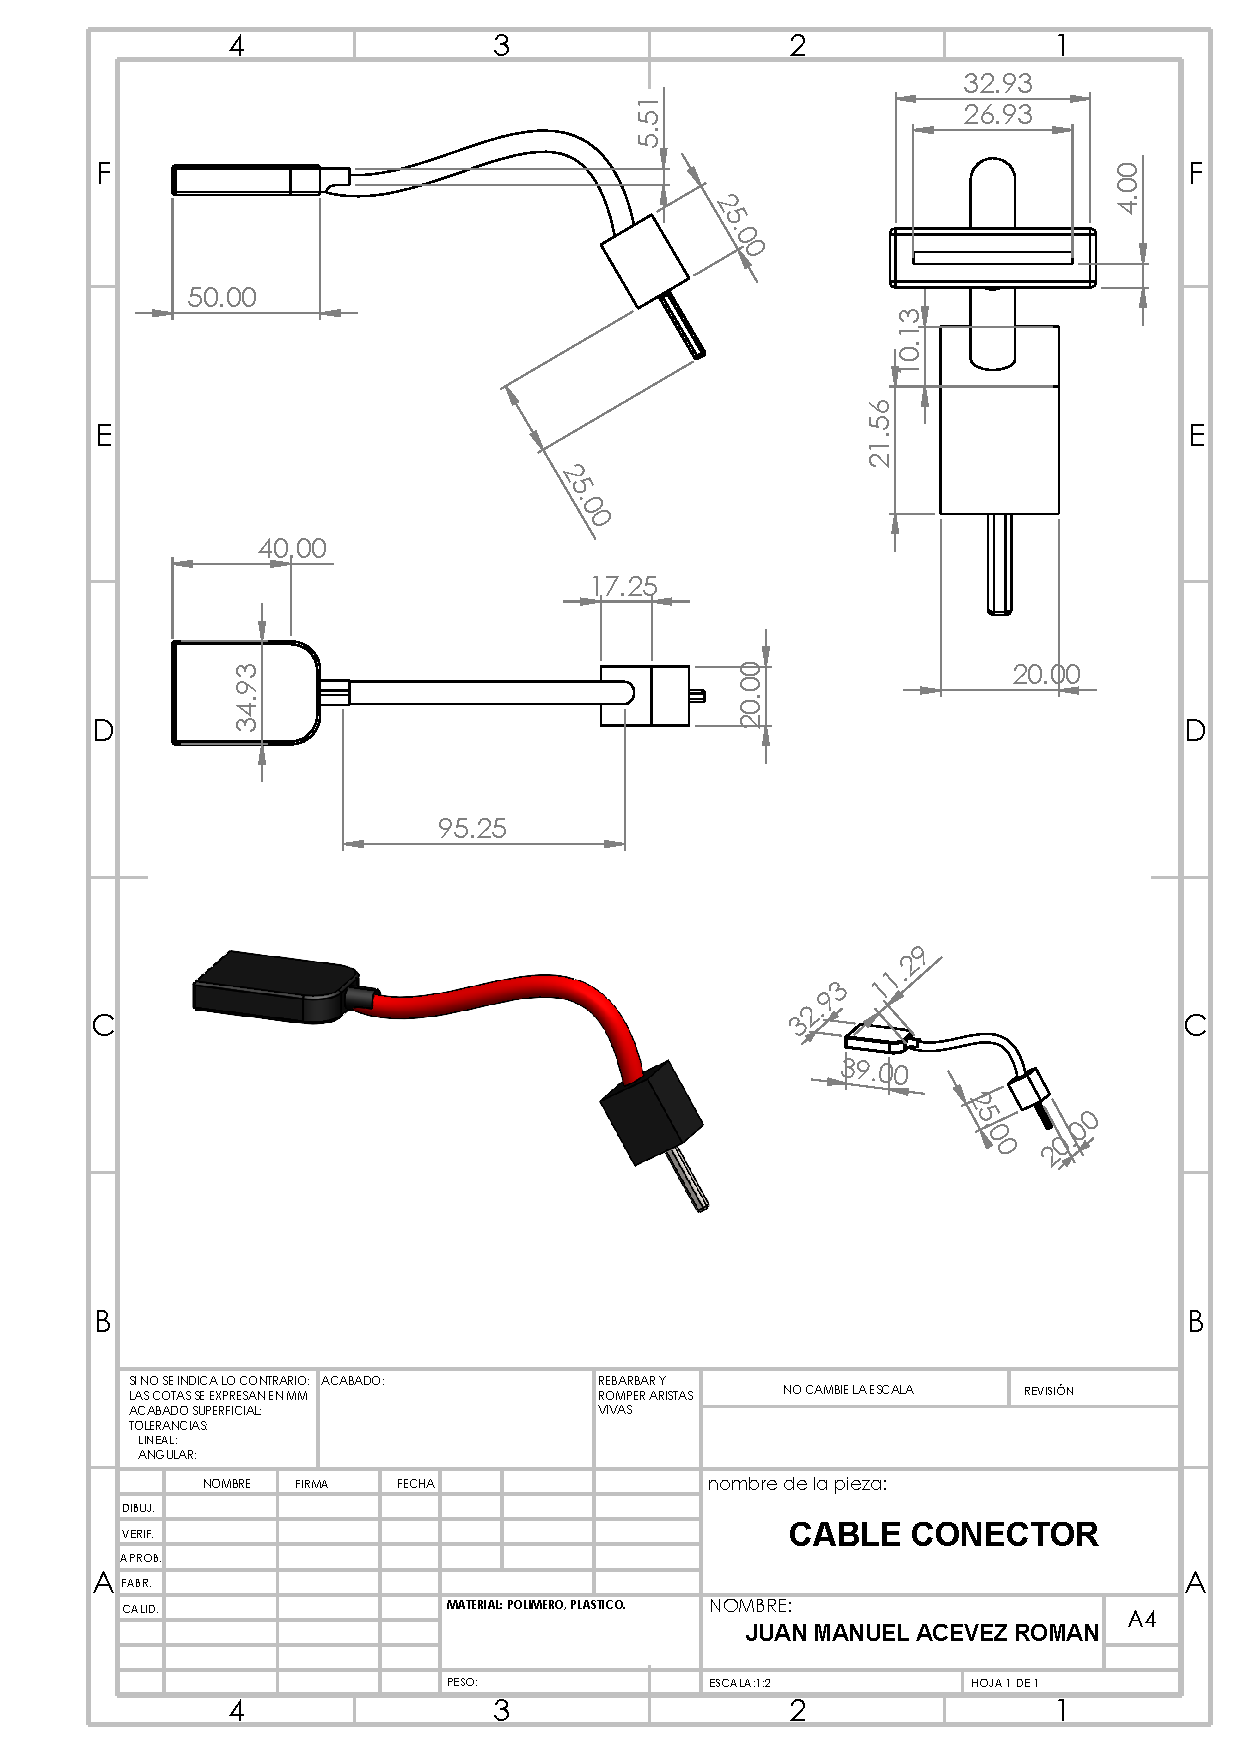
\includegraphics[height=19mm]{1/img/cable conetor.pdf}  & 
       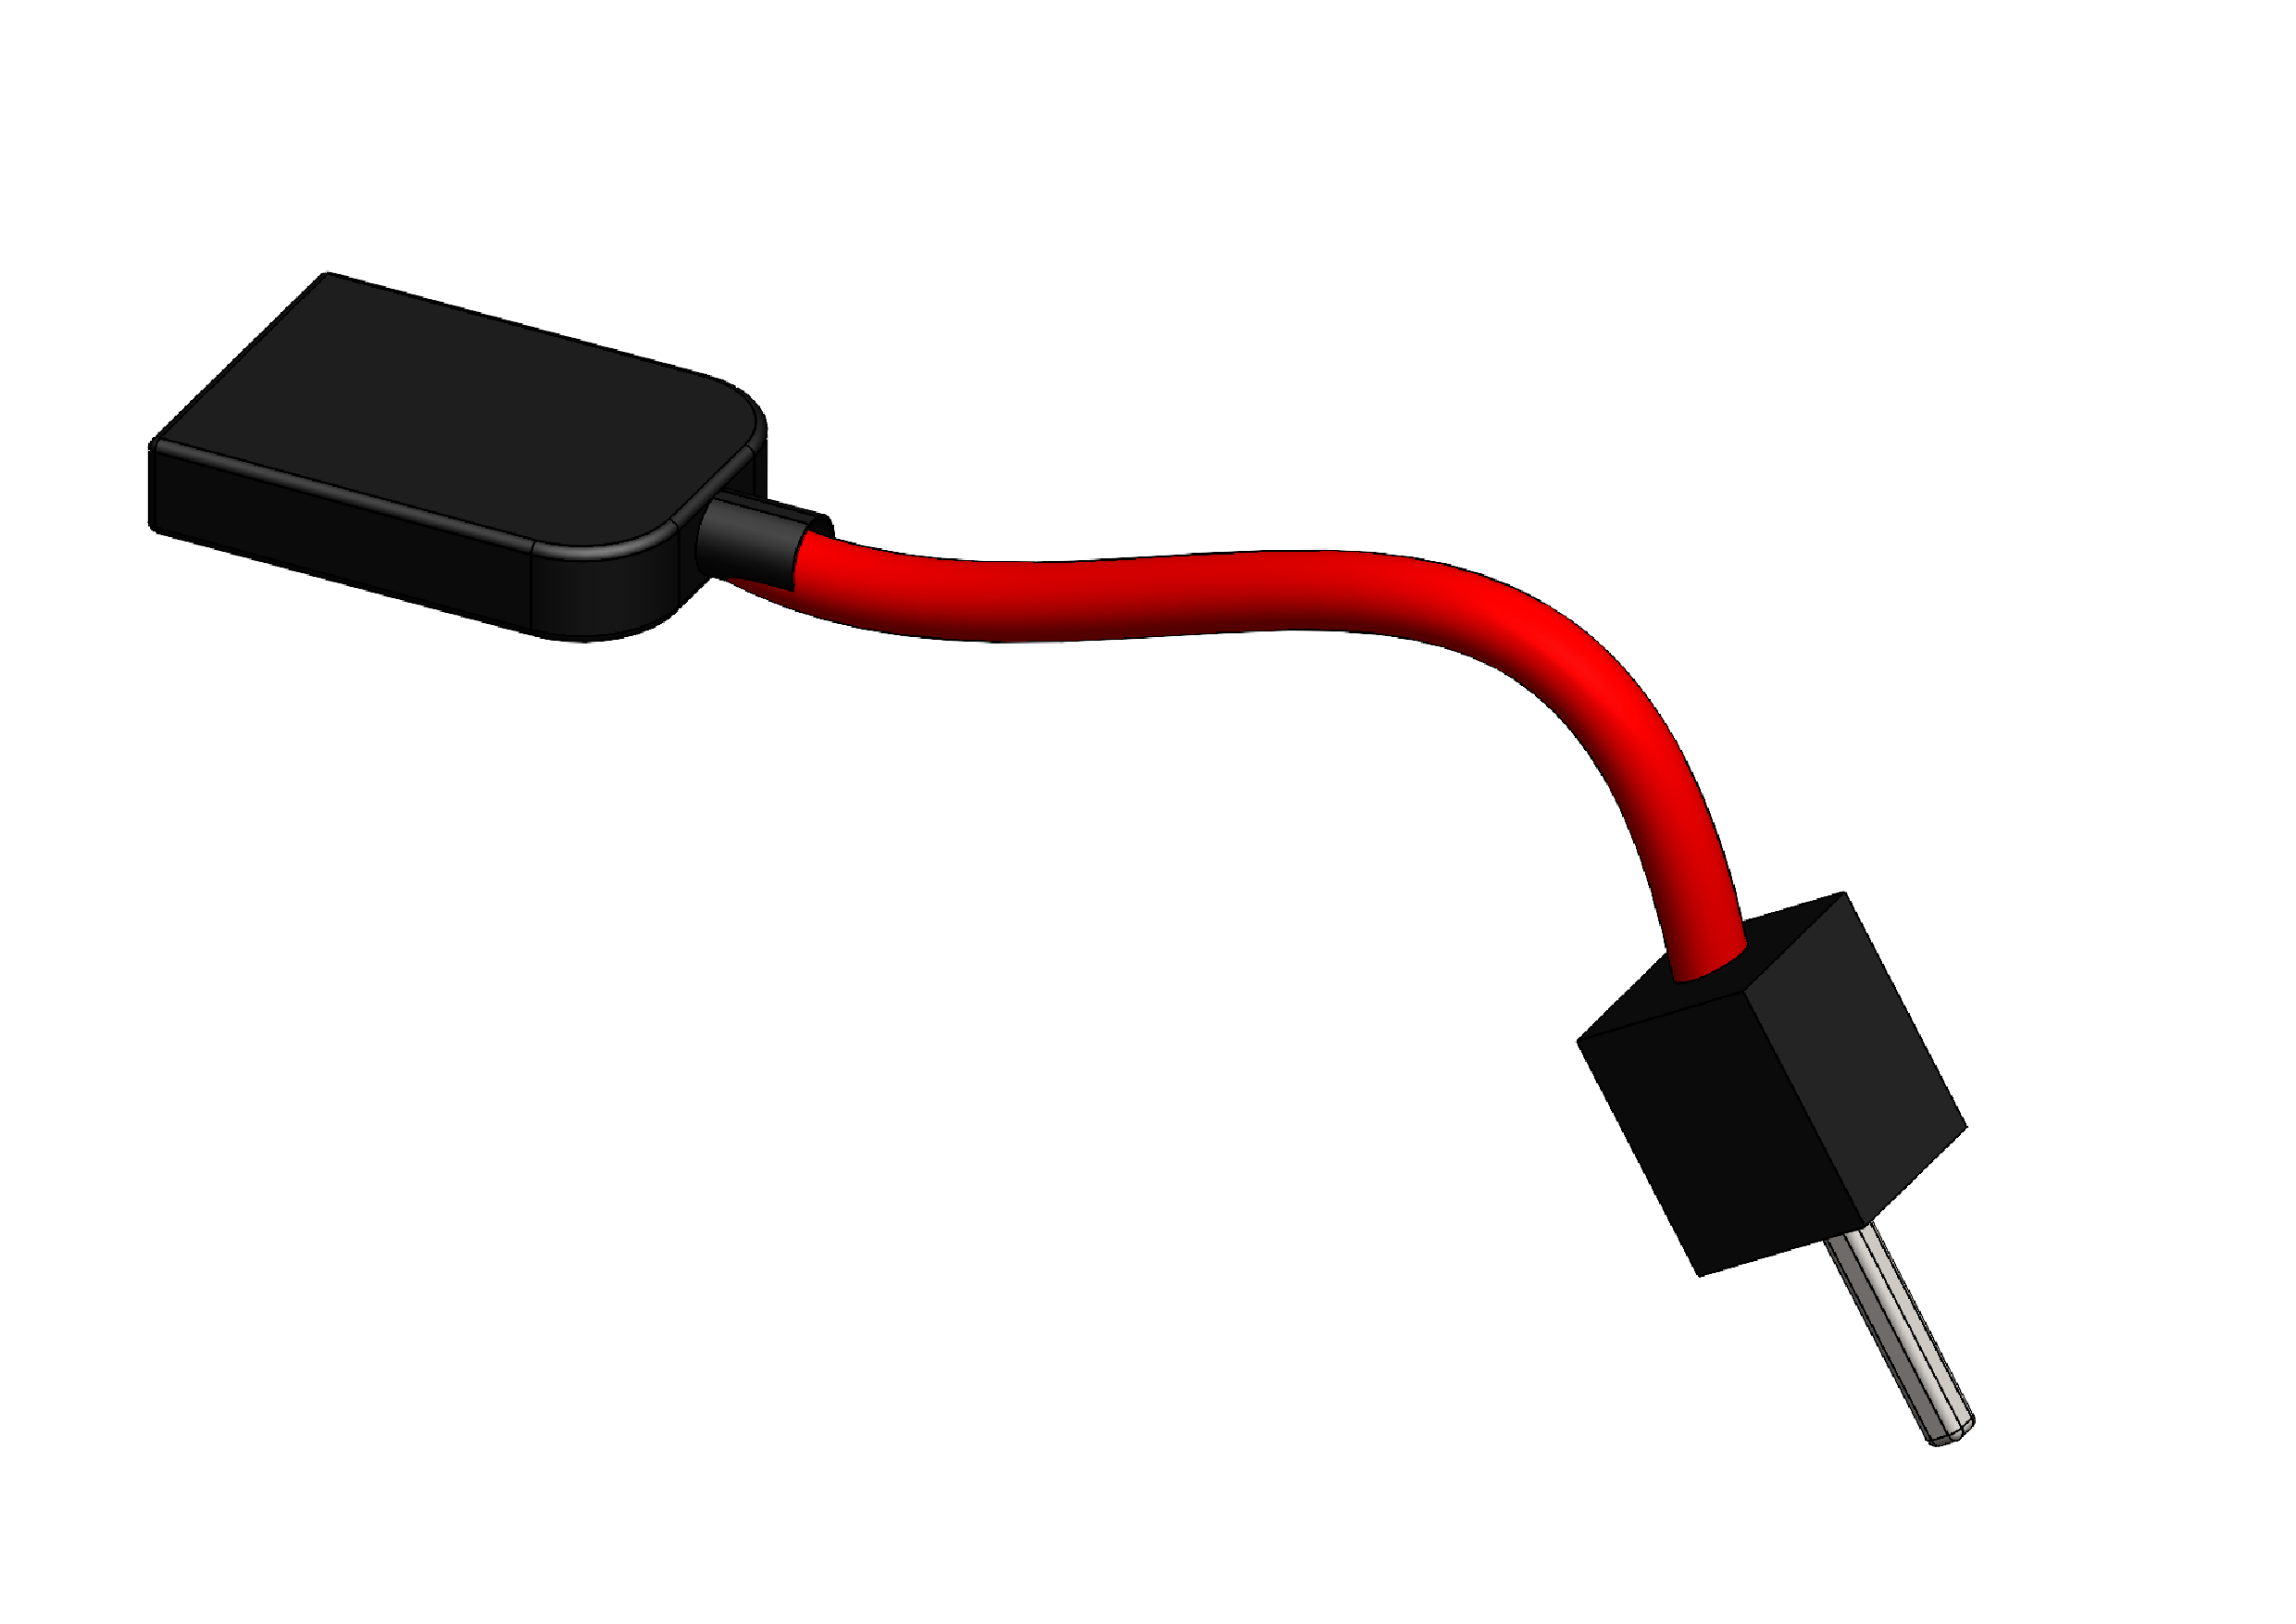
\includegraphics[width=19mm]{1/img/cable conetor_1.pdf} \\
        \hline
        Cable tipo C &  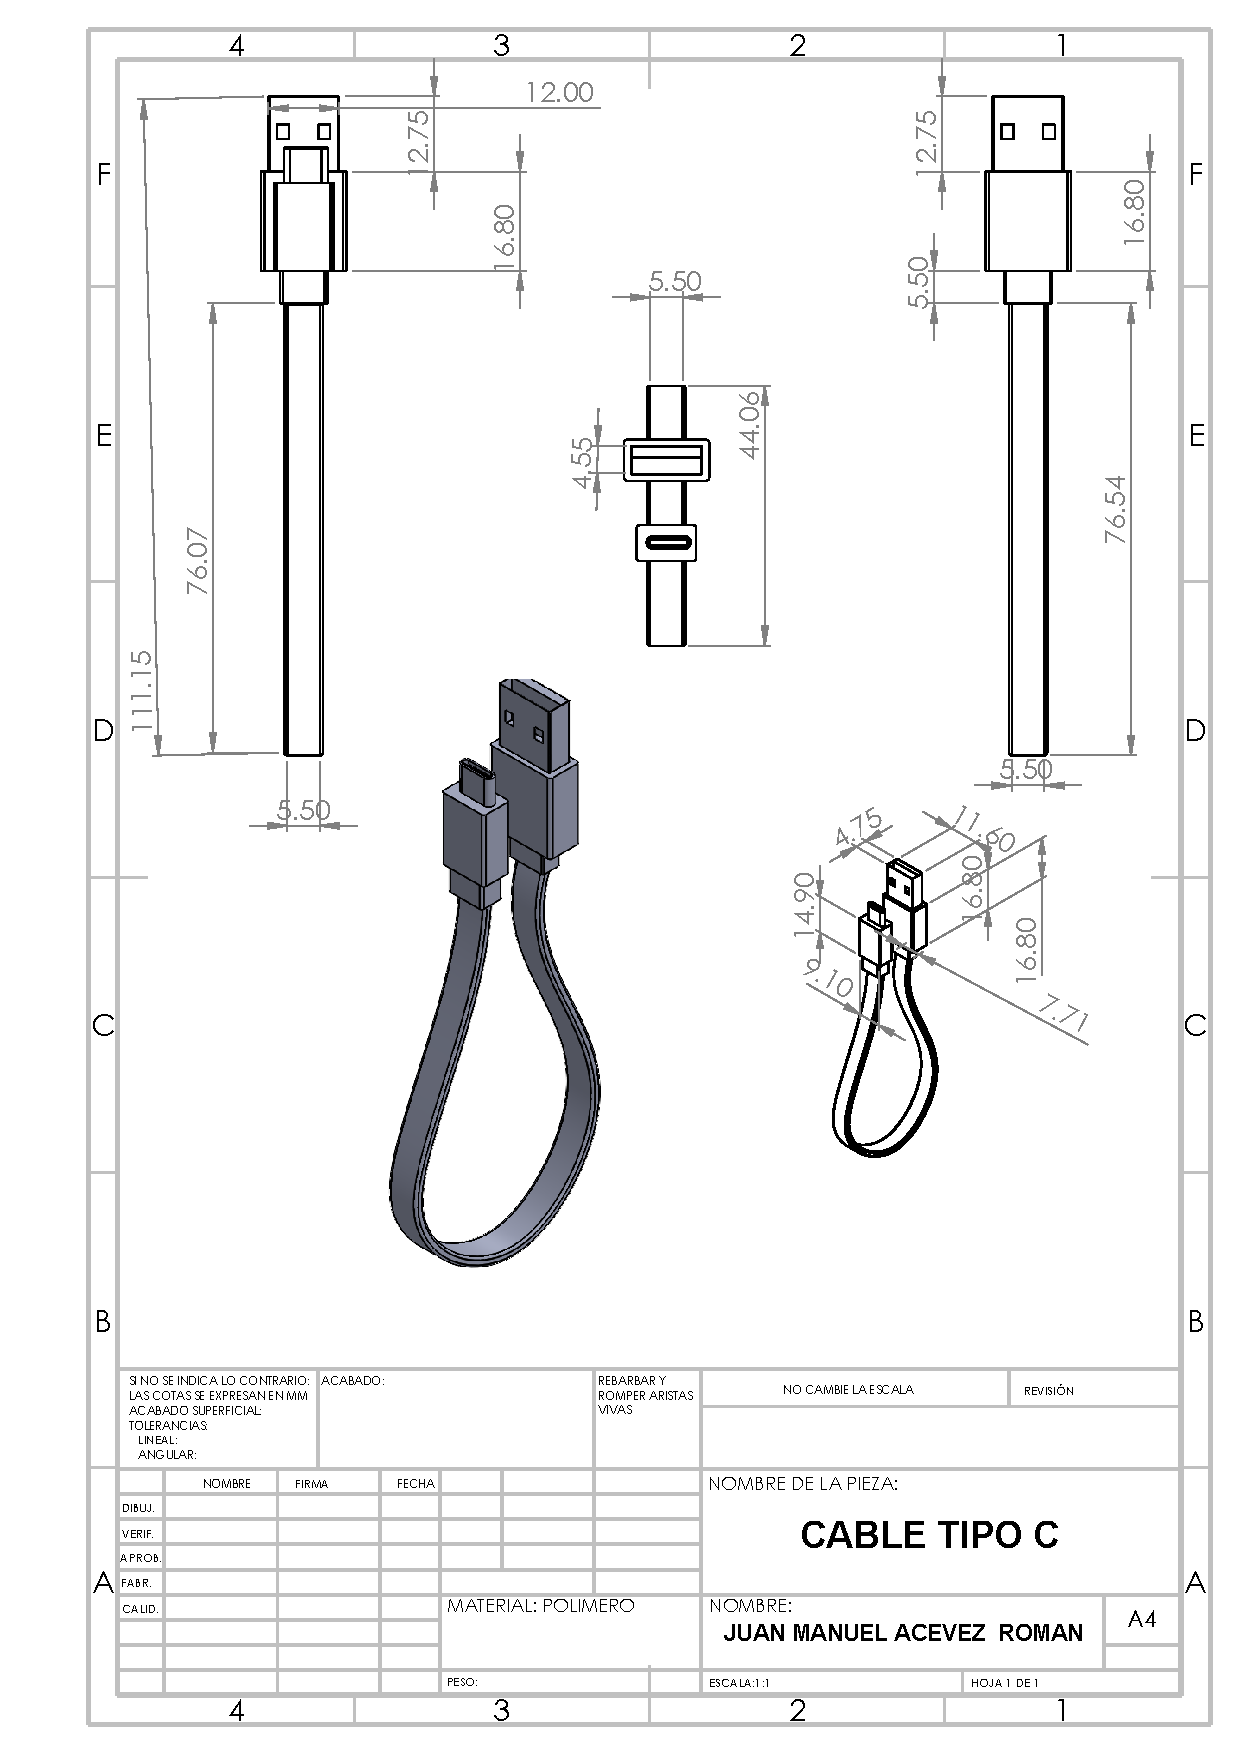
\includegraphics[height=19mm]{1/img/Cable tipo C.pdf}  & 
       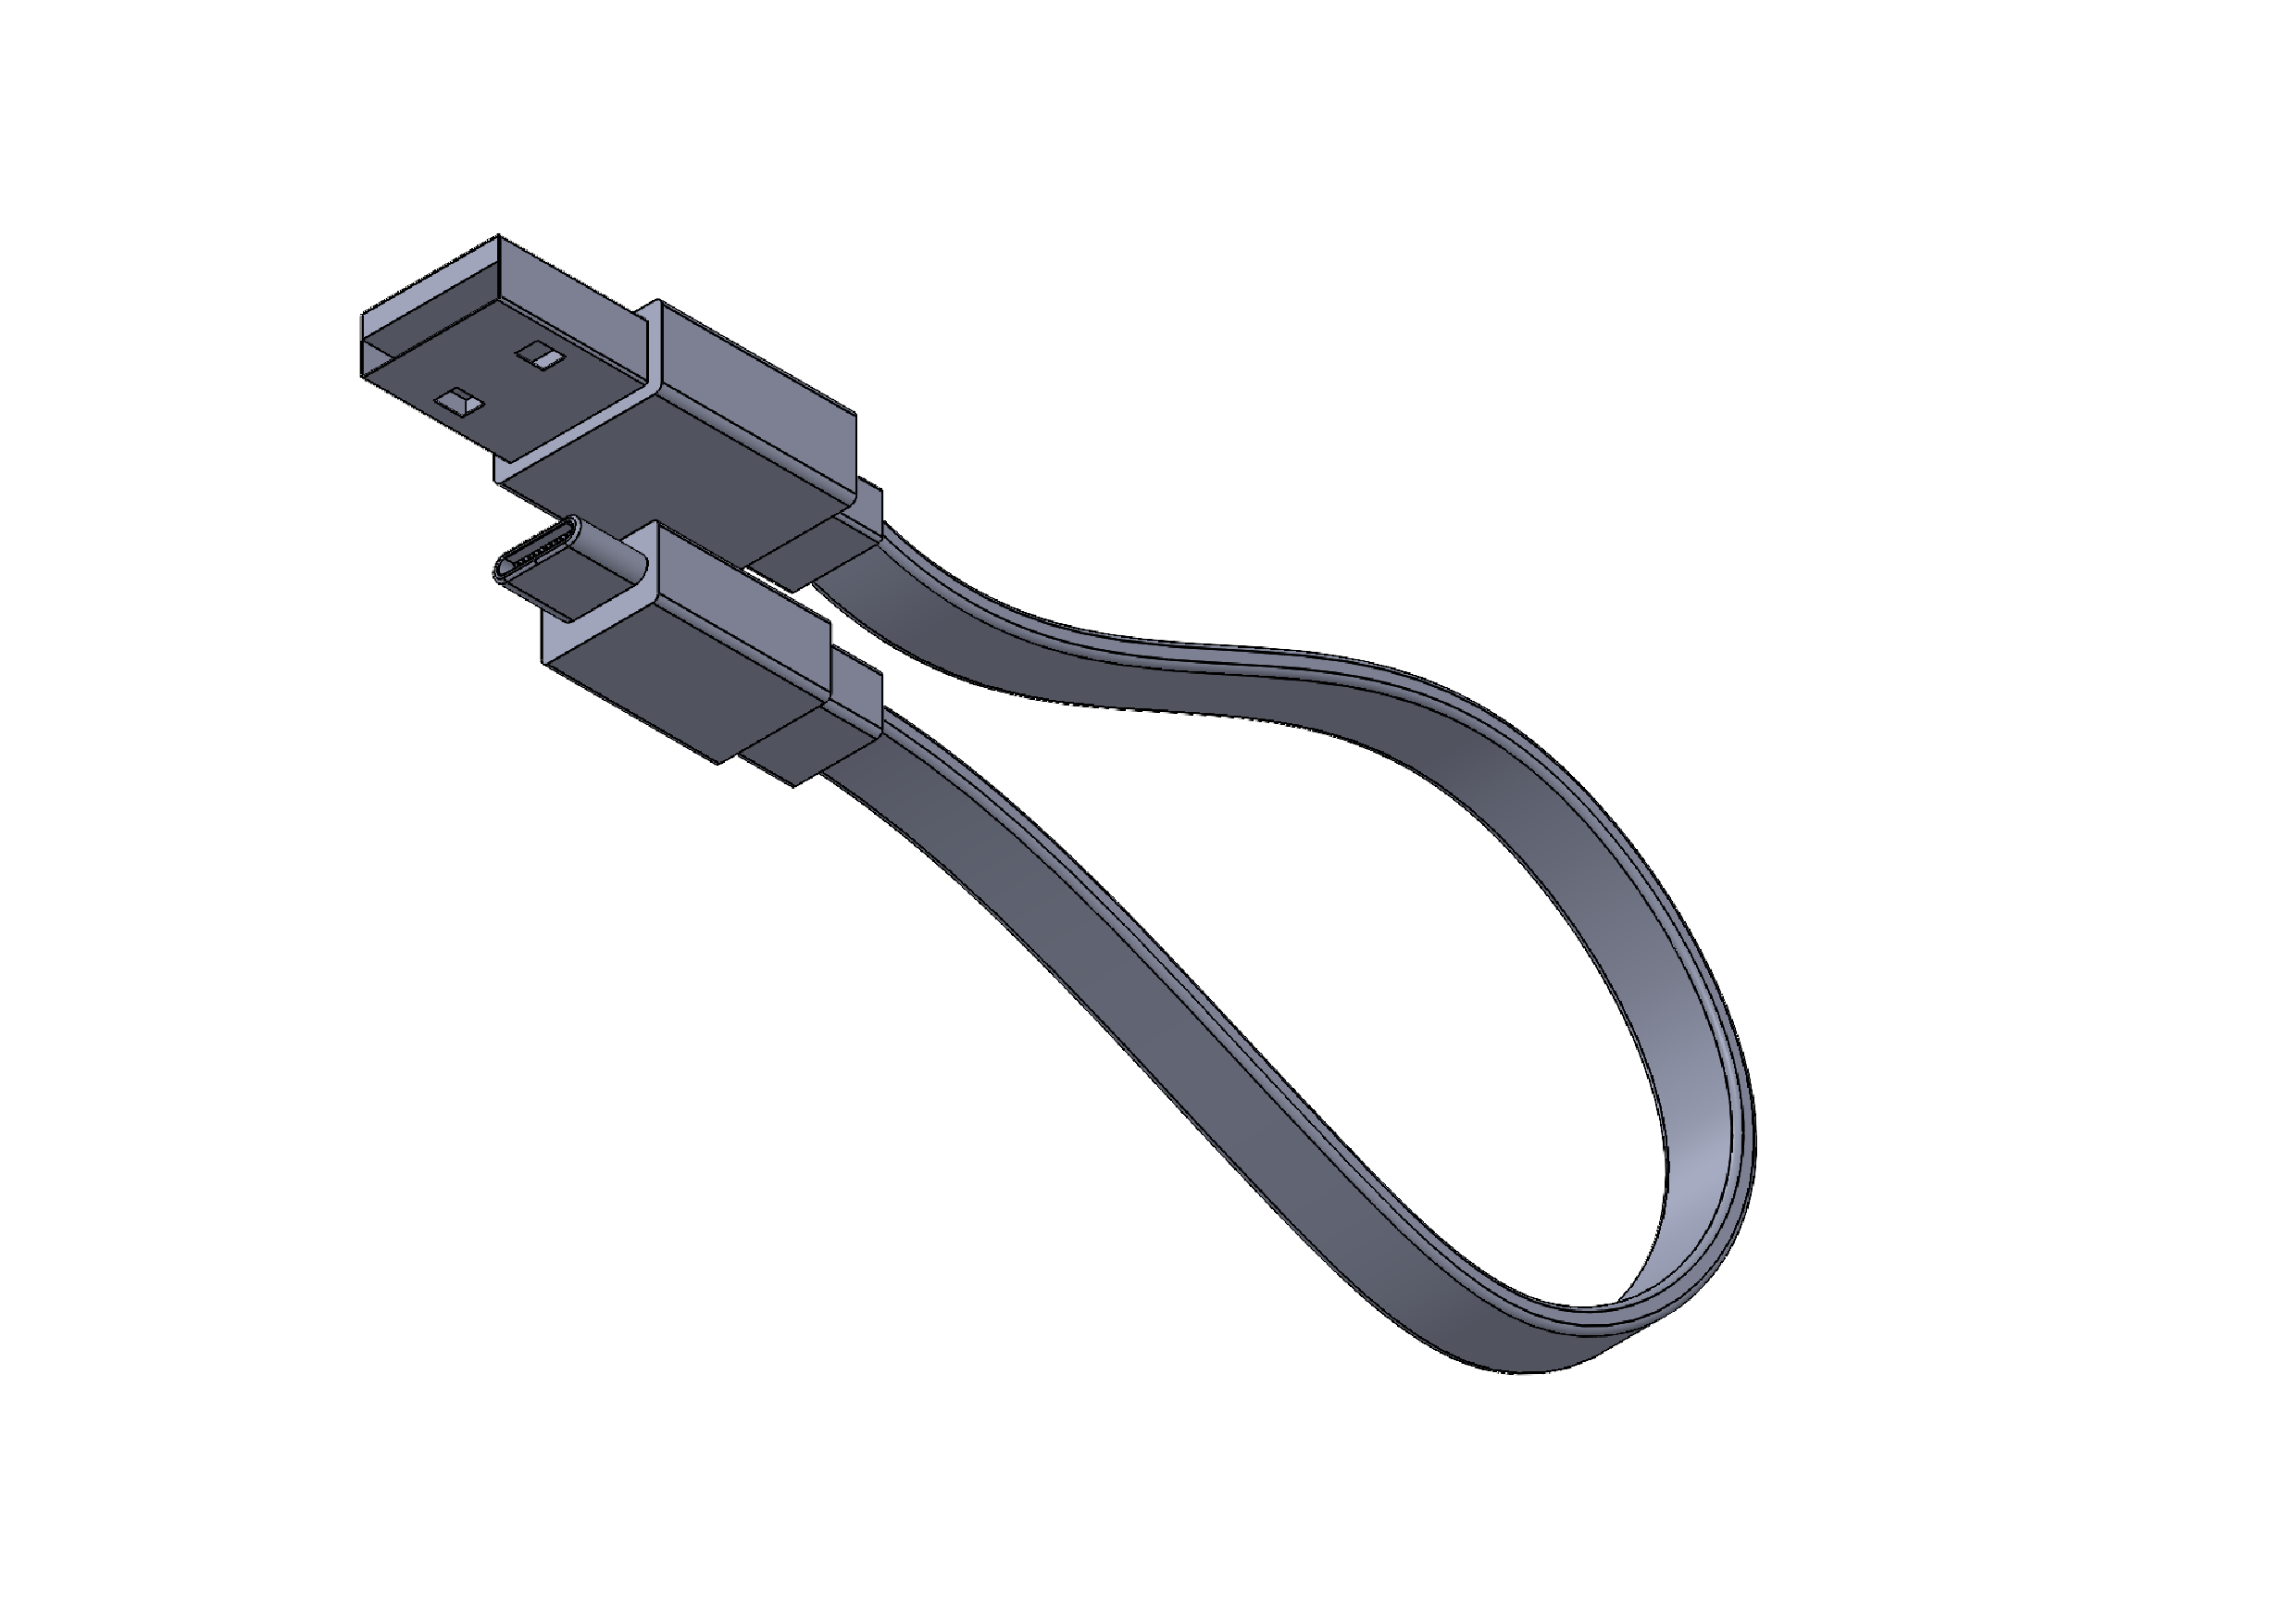
\includegraphics[width=19mm]{1/img/Cable tipo C_1.pdf} \\
        \hline
      Protoboard &  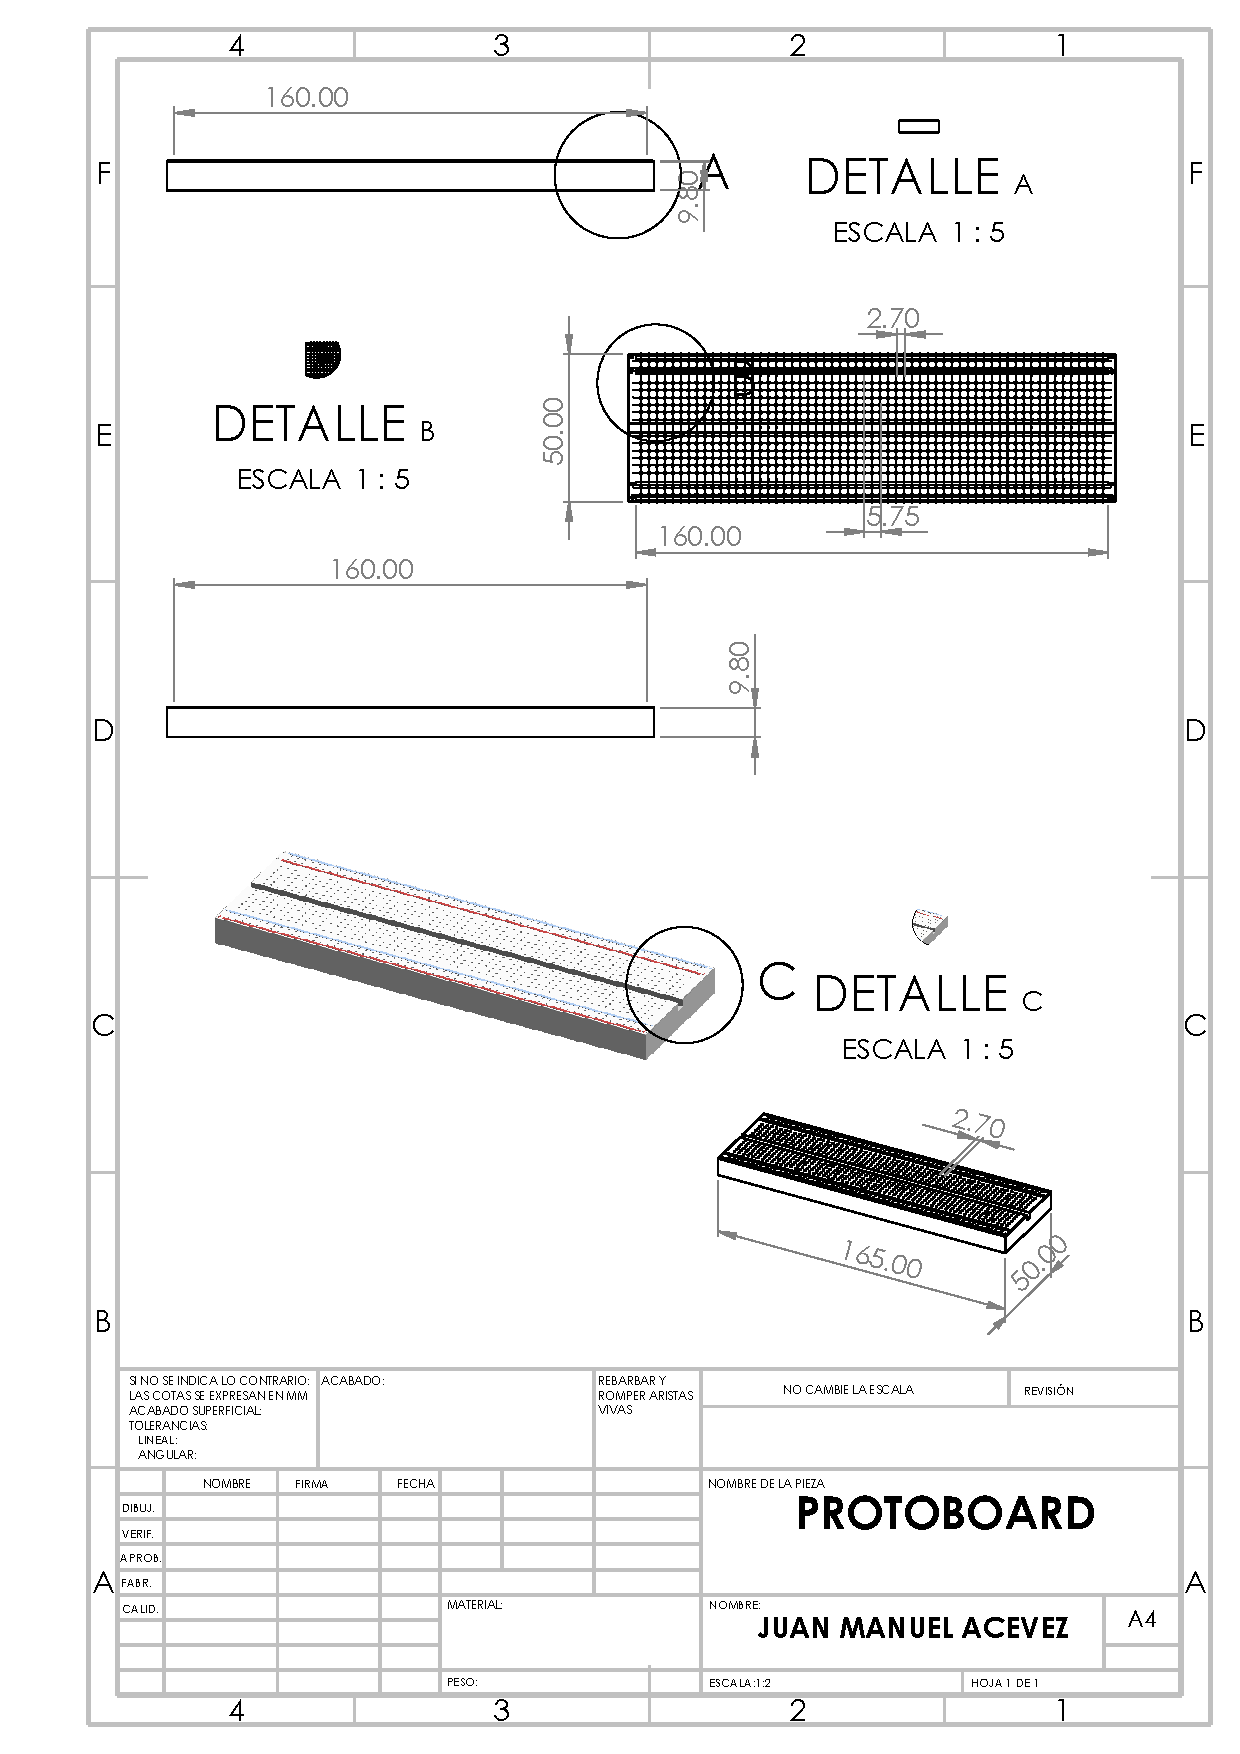
\includegraphics[height=19mm]{1/img/Protoboard.pdf}  & 
       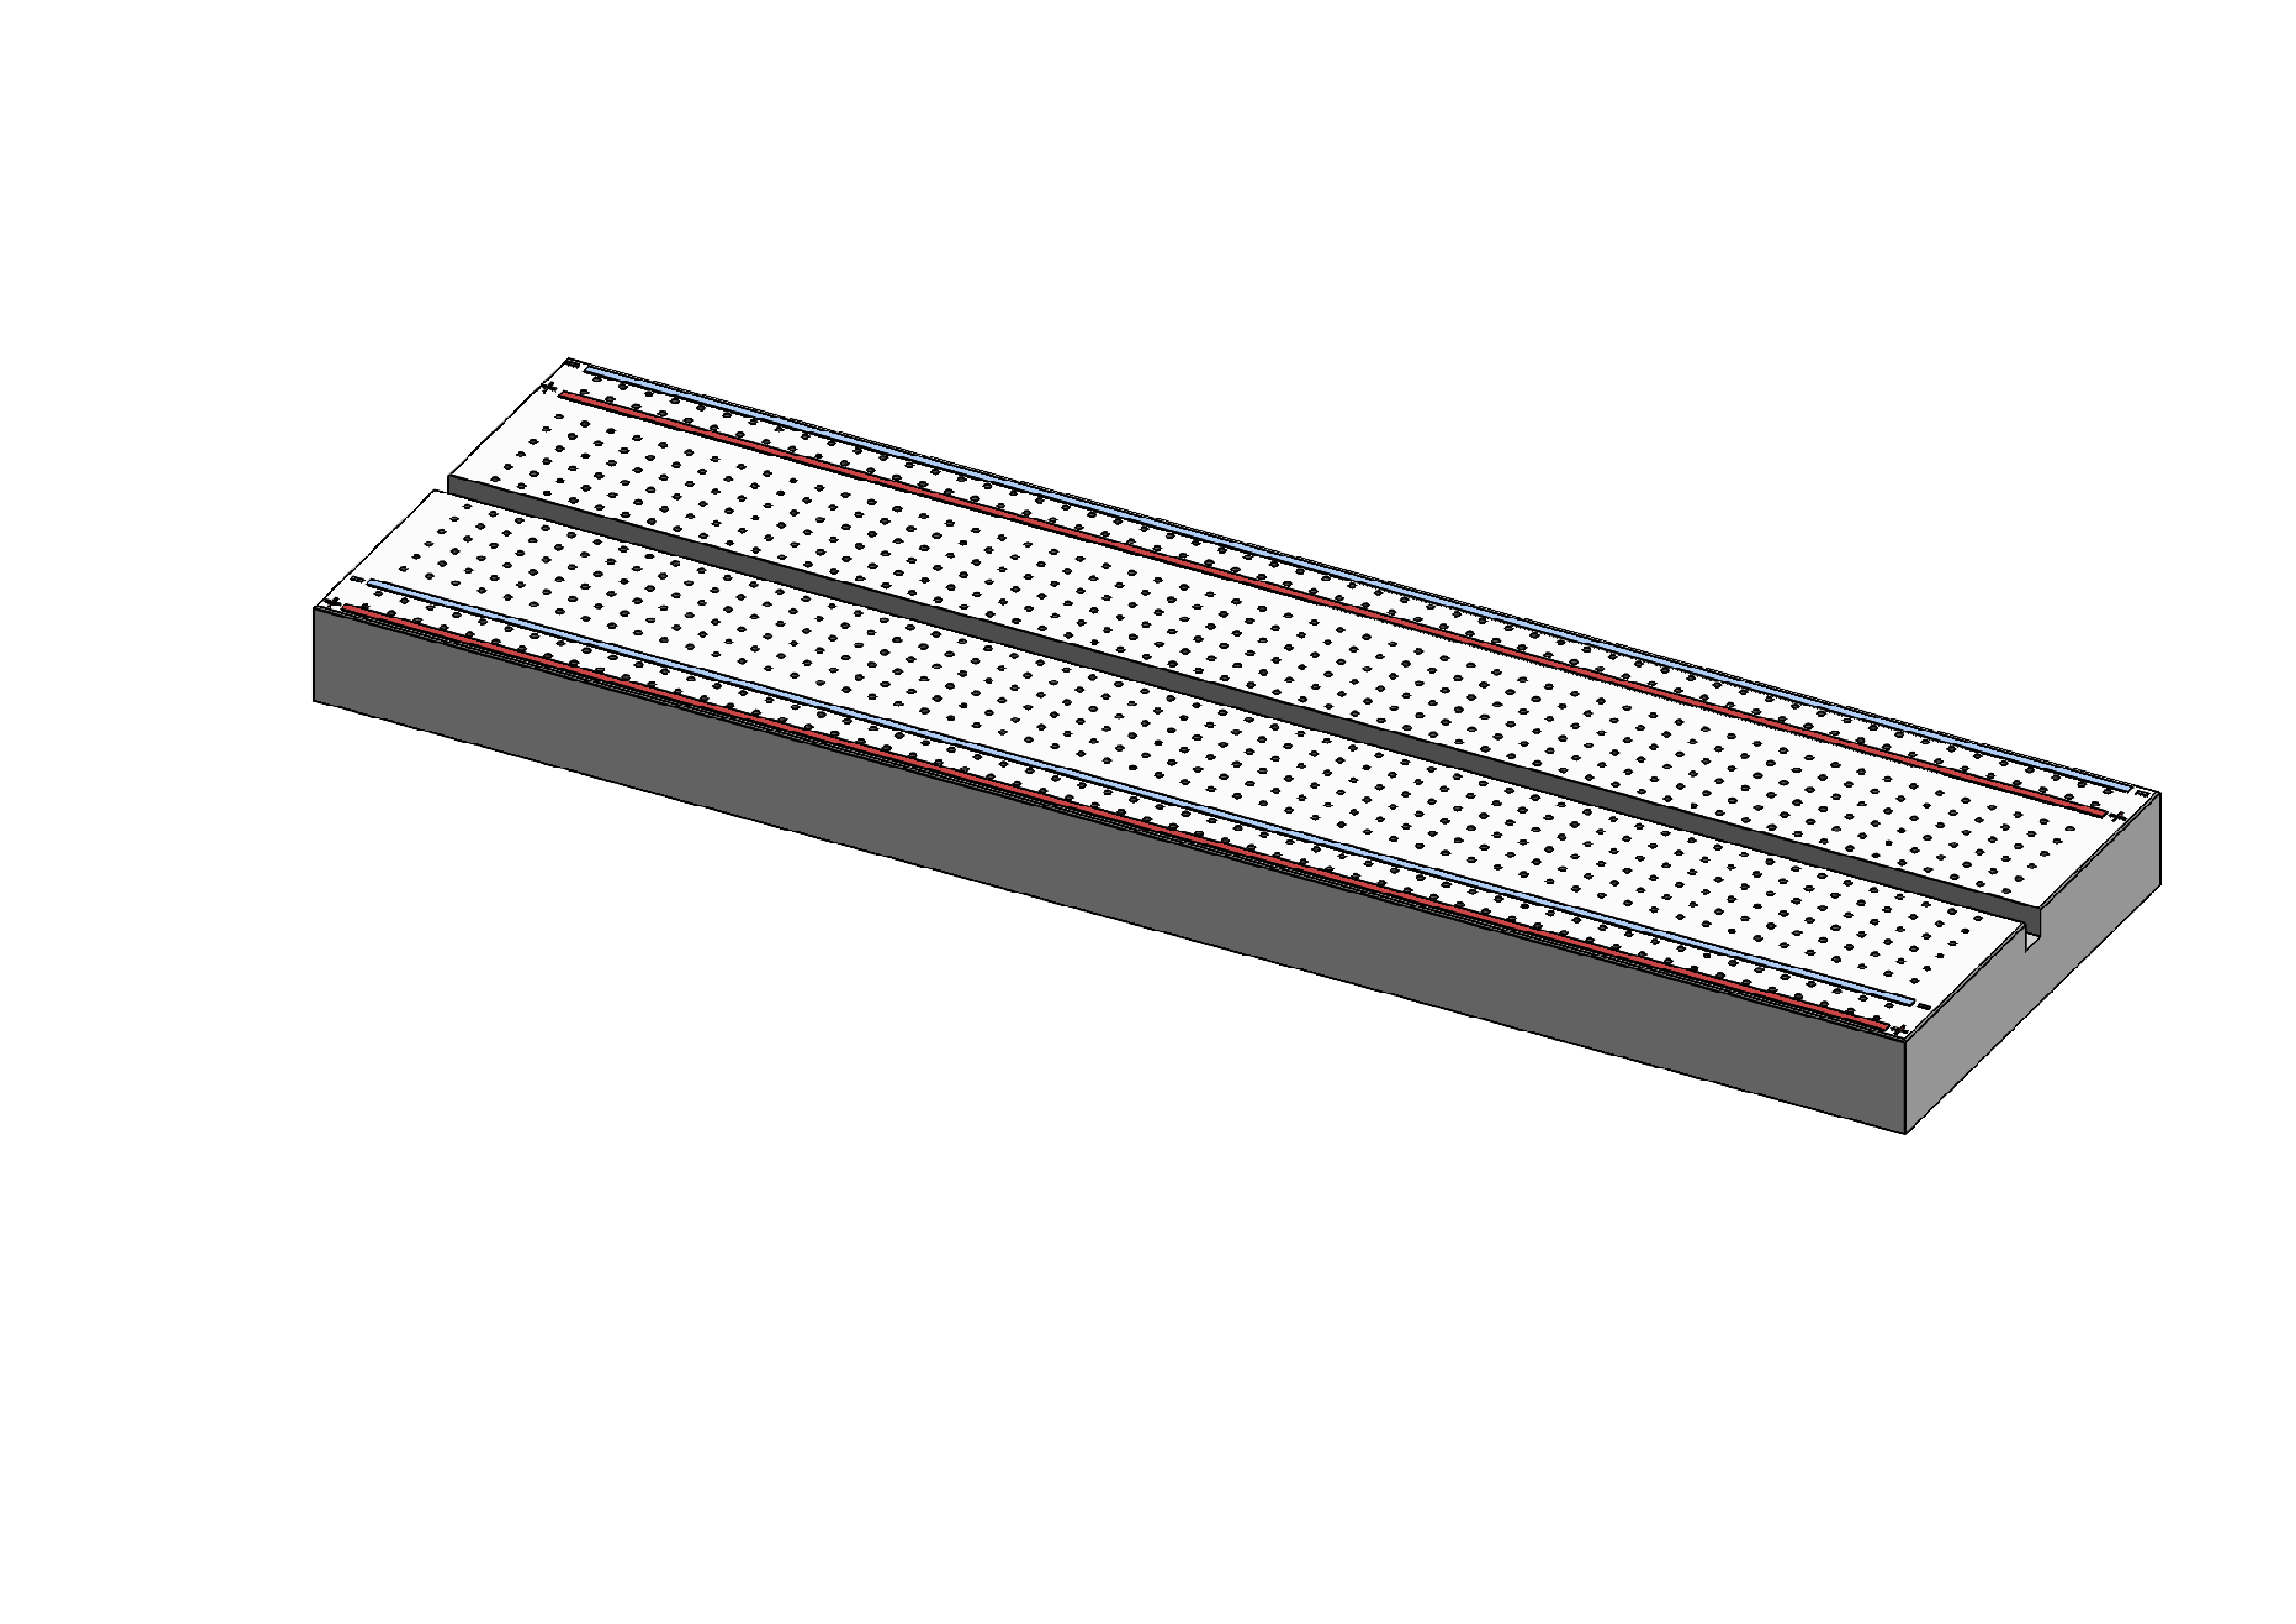
\includegraphics[width=19mm]{1/img/Protoboard_1.pdf} \\
        \hline
       Conetor &  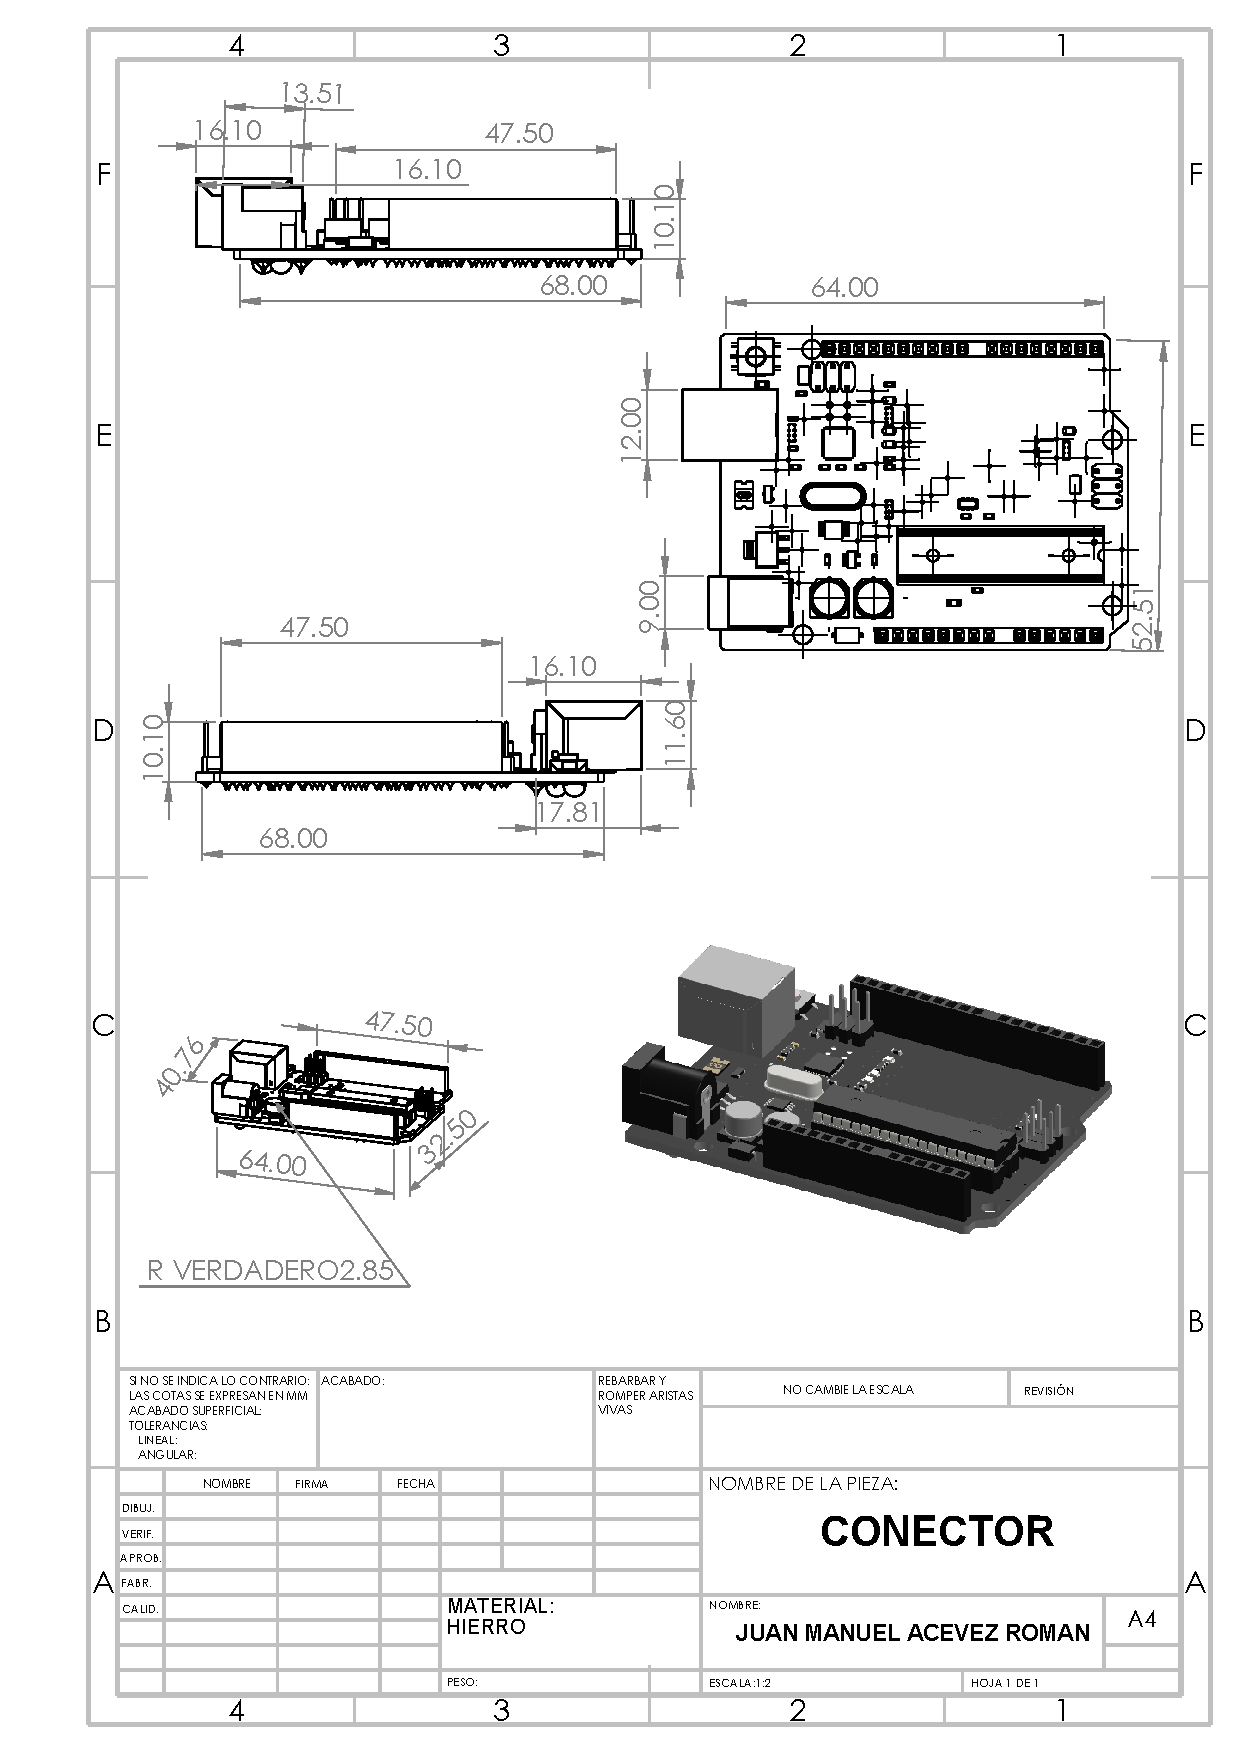
\includegraphics[height=19mm]{1/img/Conector.pdf}  & 
       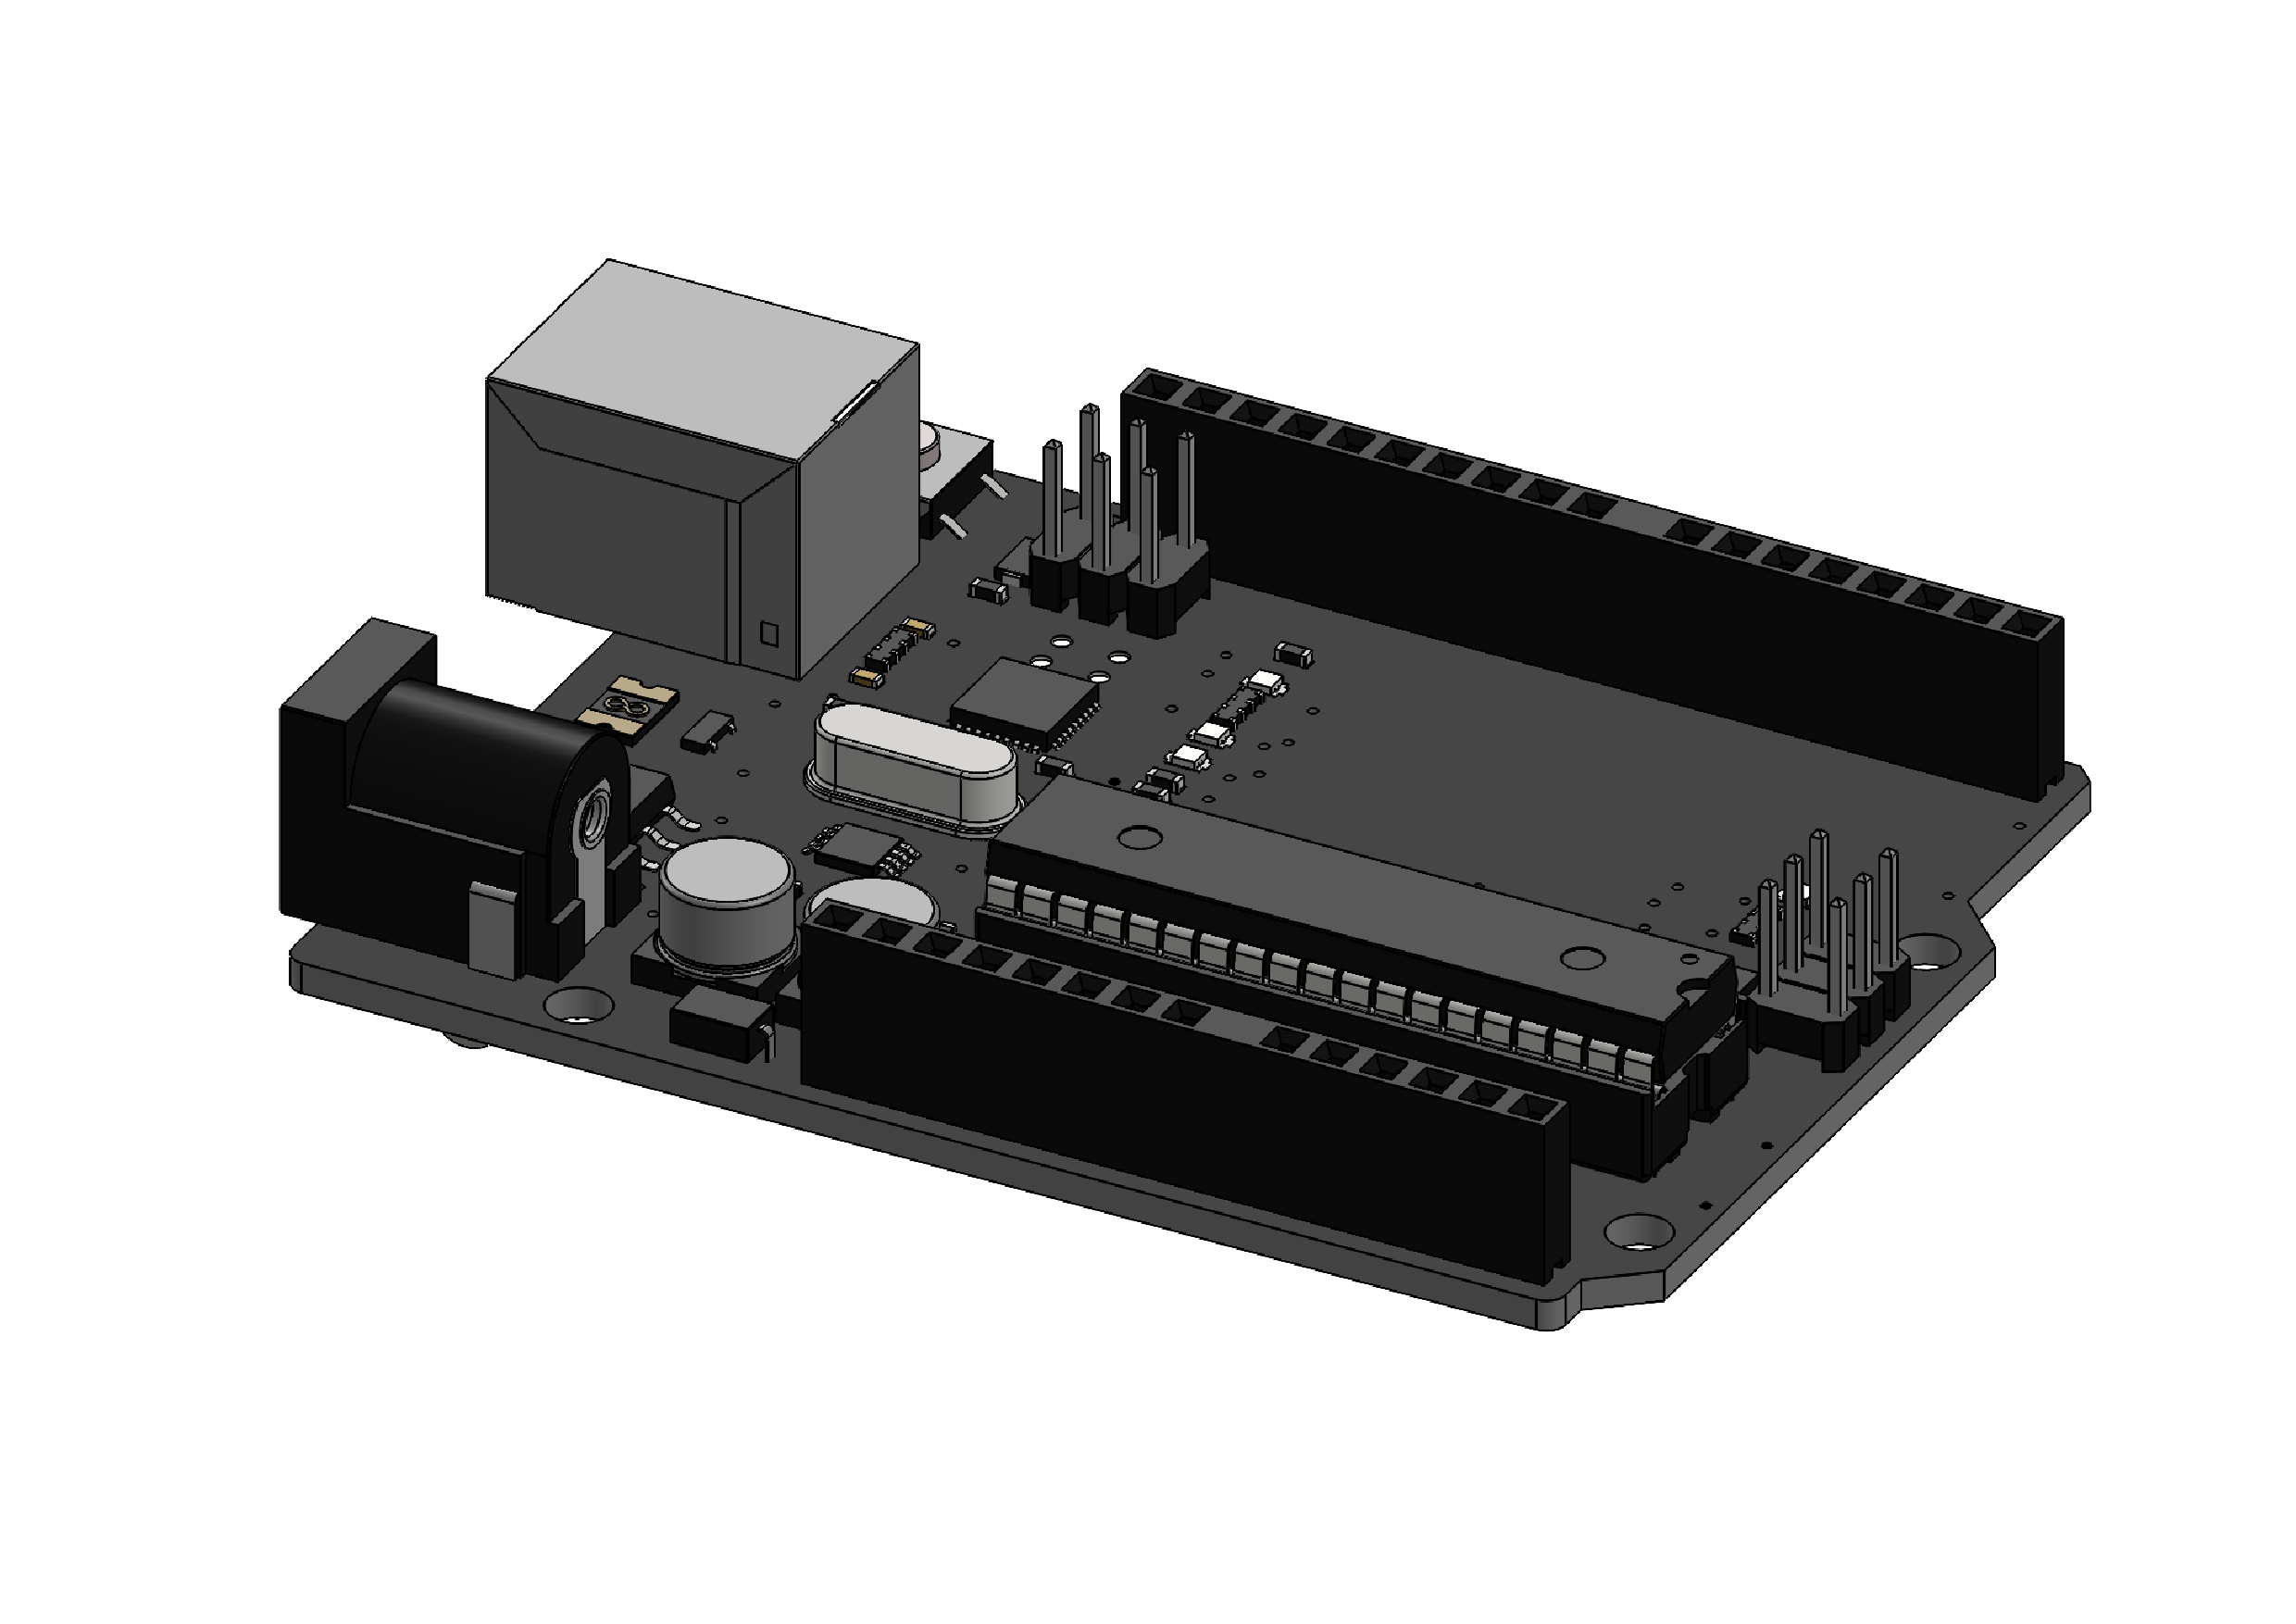
\includegraphics[width=19mm]{1/img/Conector_1.pdf} \\
        \hline
        Multicontacto &  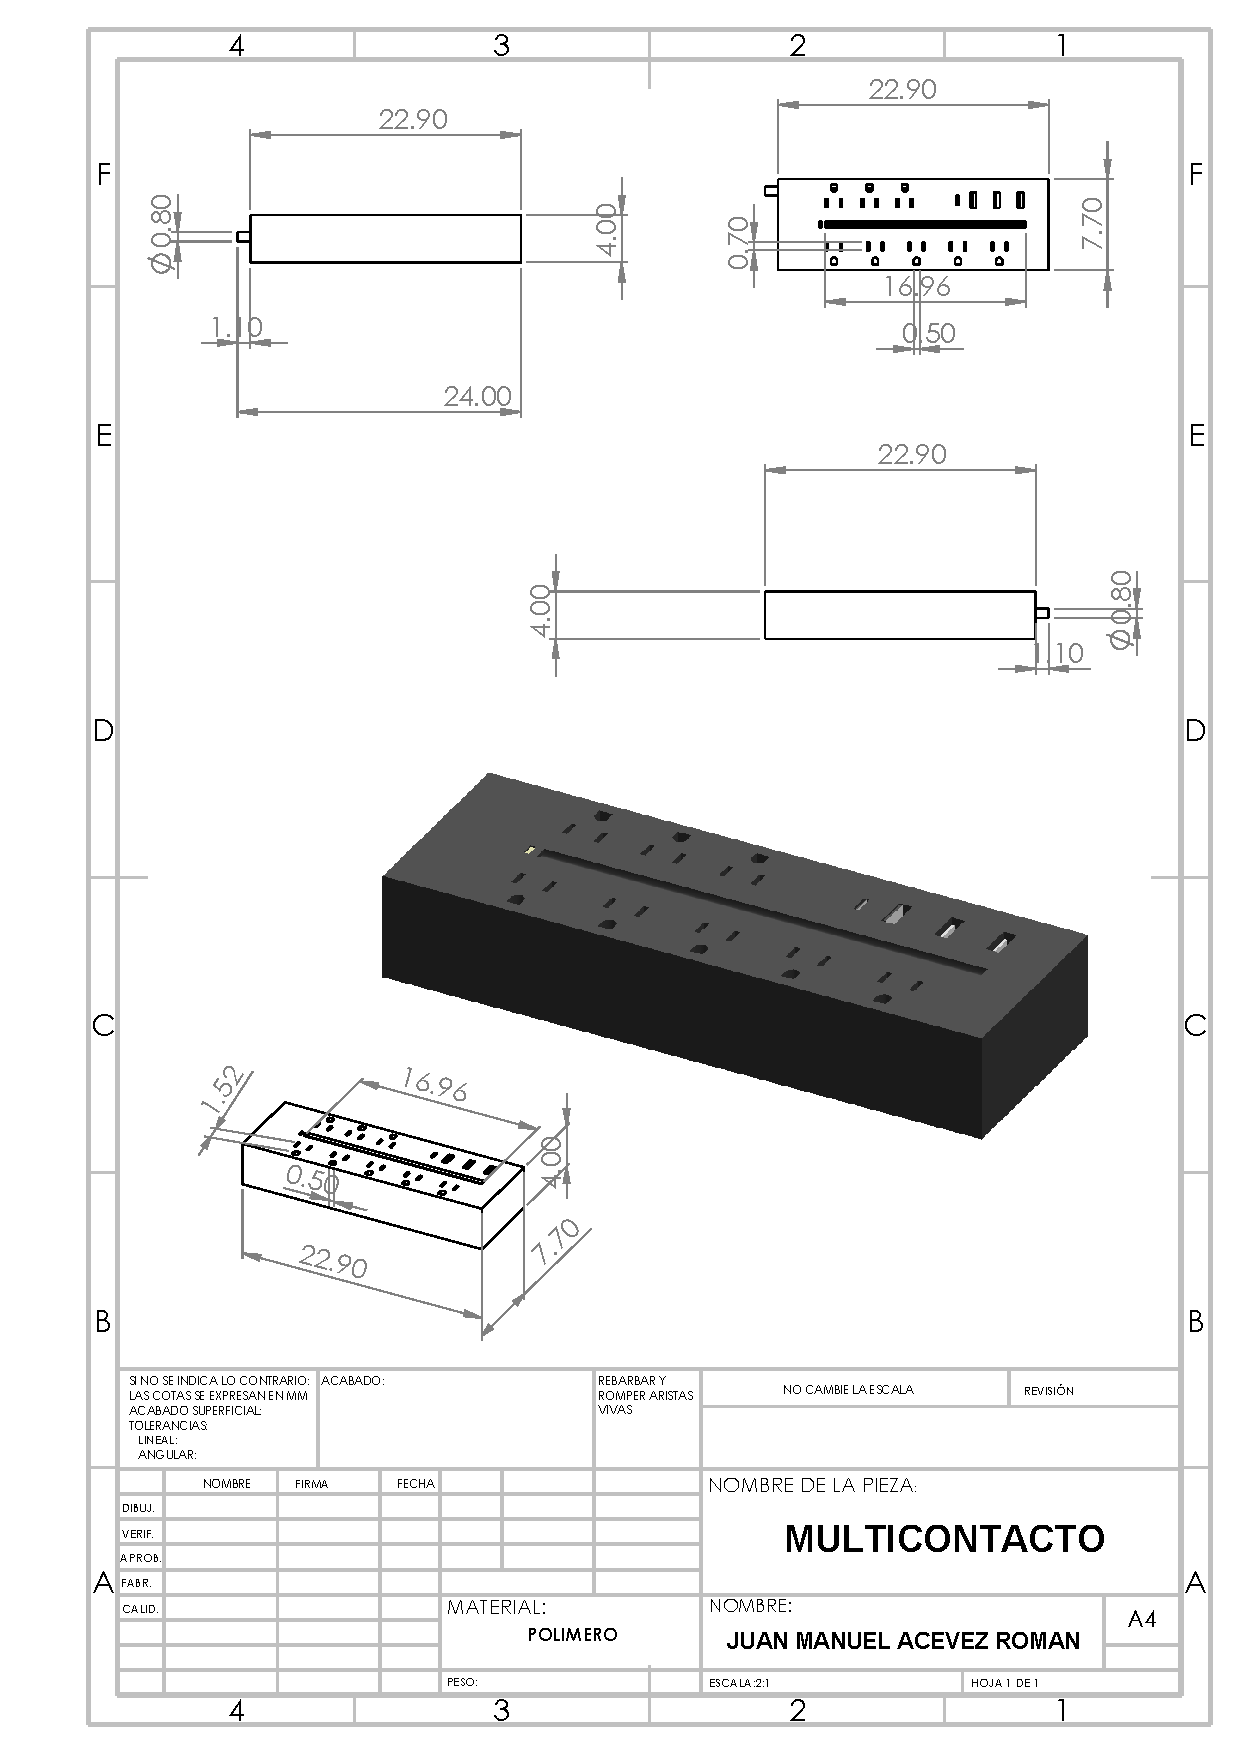
\includegraphics[height=19mm]{1/img/Multicontacto.pdf}  & 
       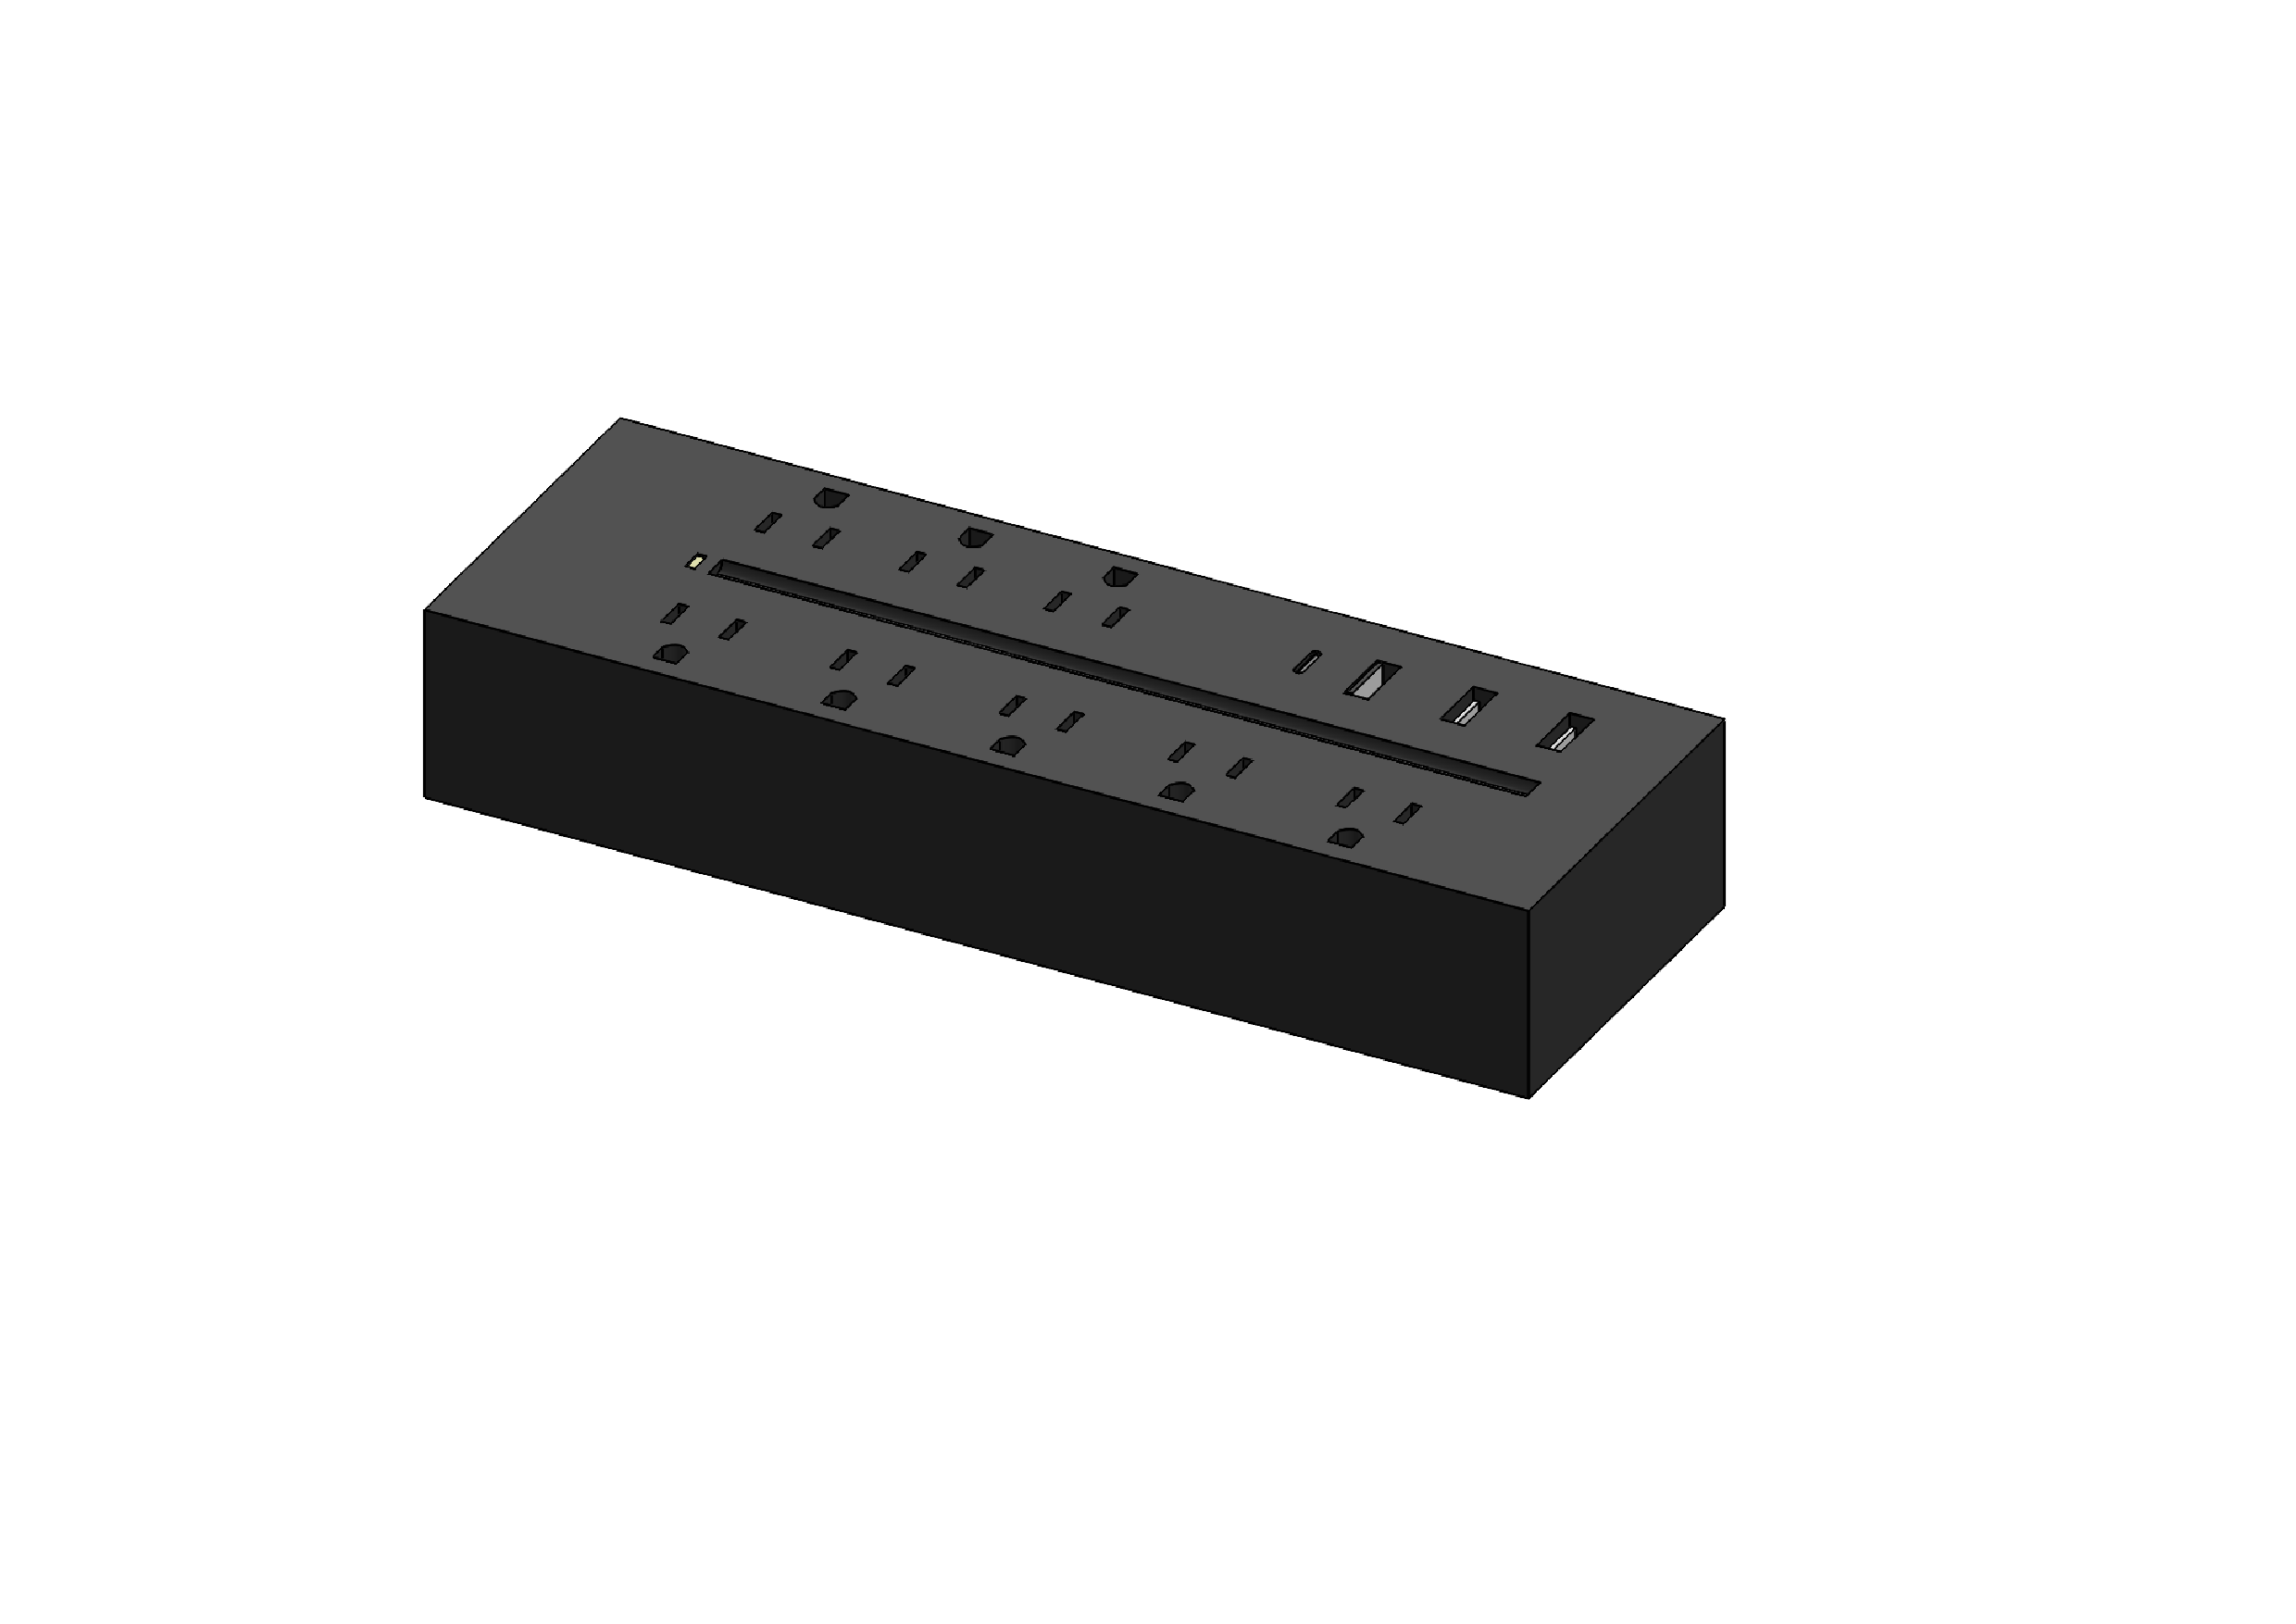
\includegraphics[width=19mm]{1/img/Multicontacto_1.pdf} \\
        \hline
        Pantalla led & 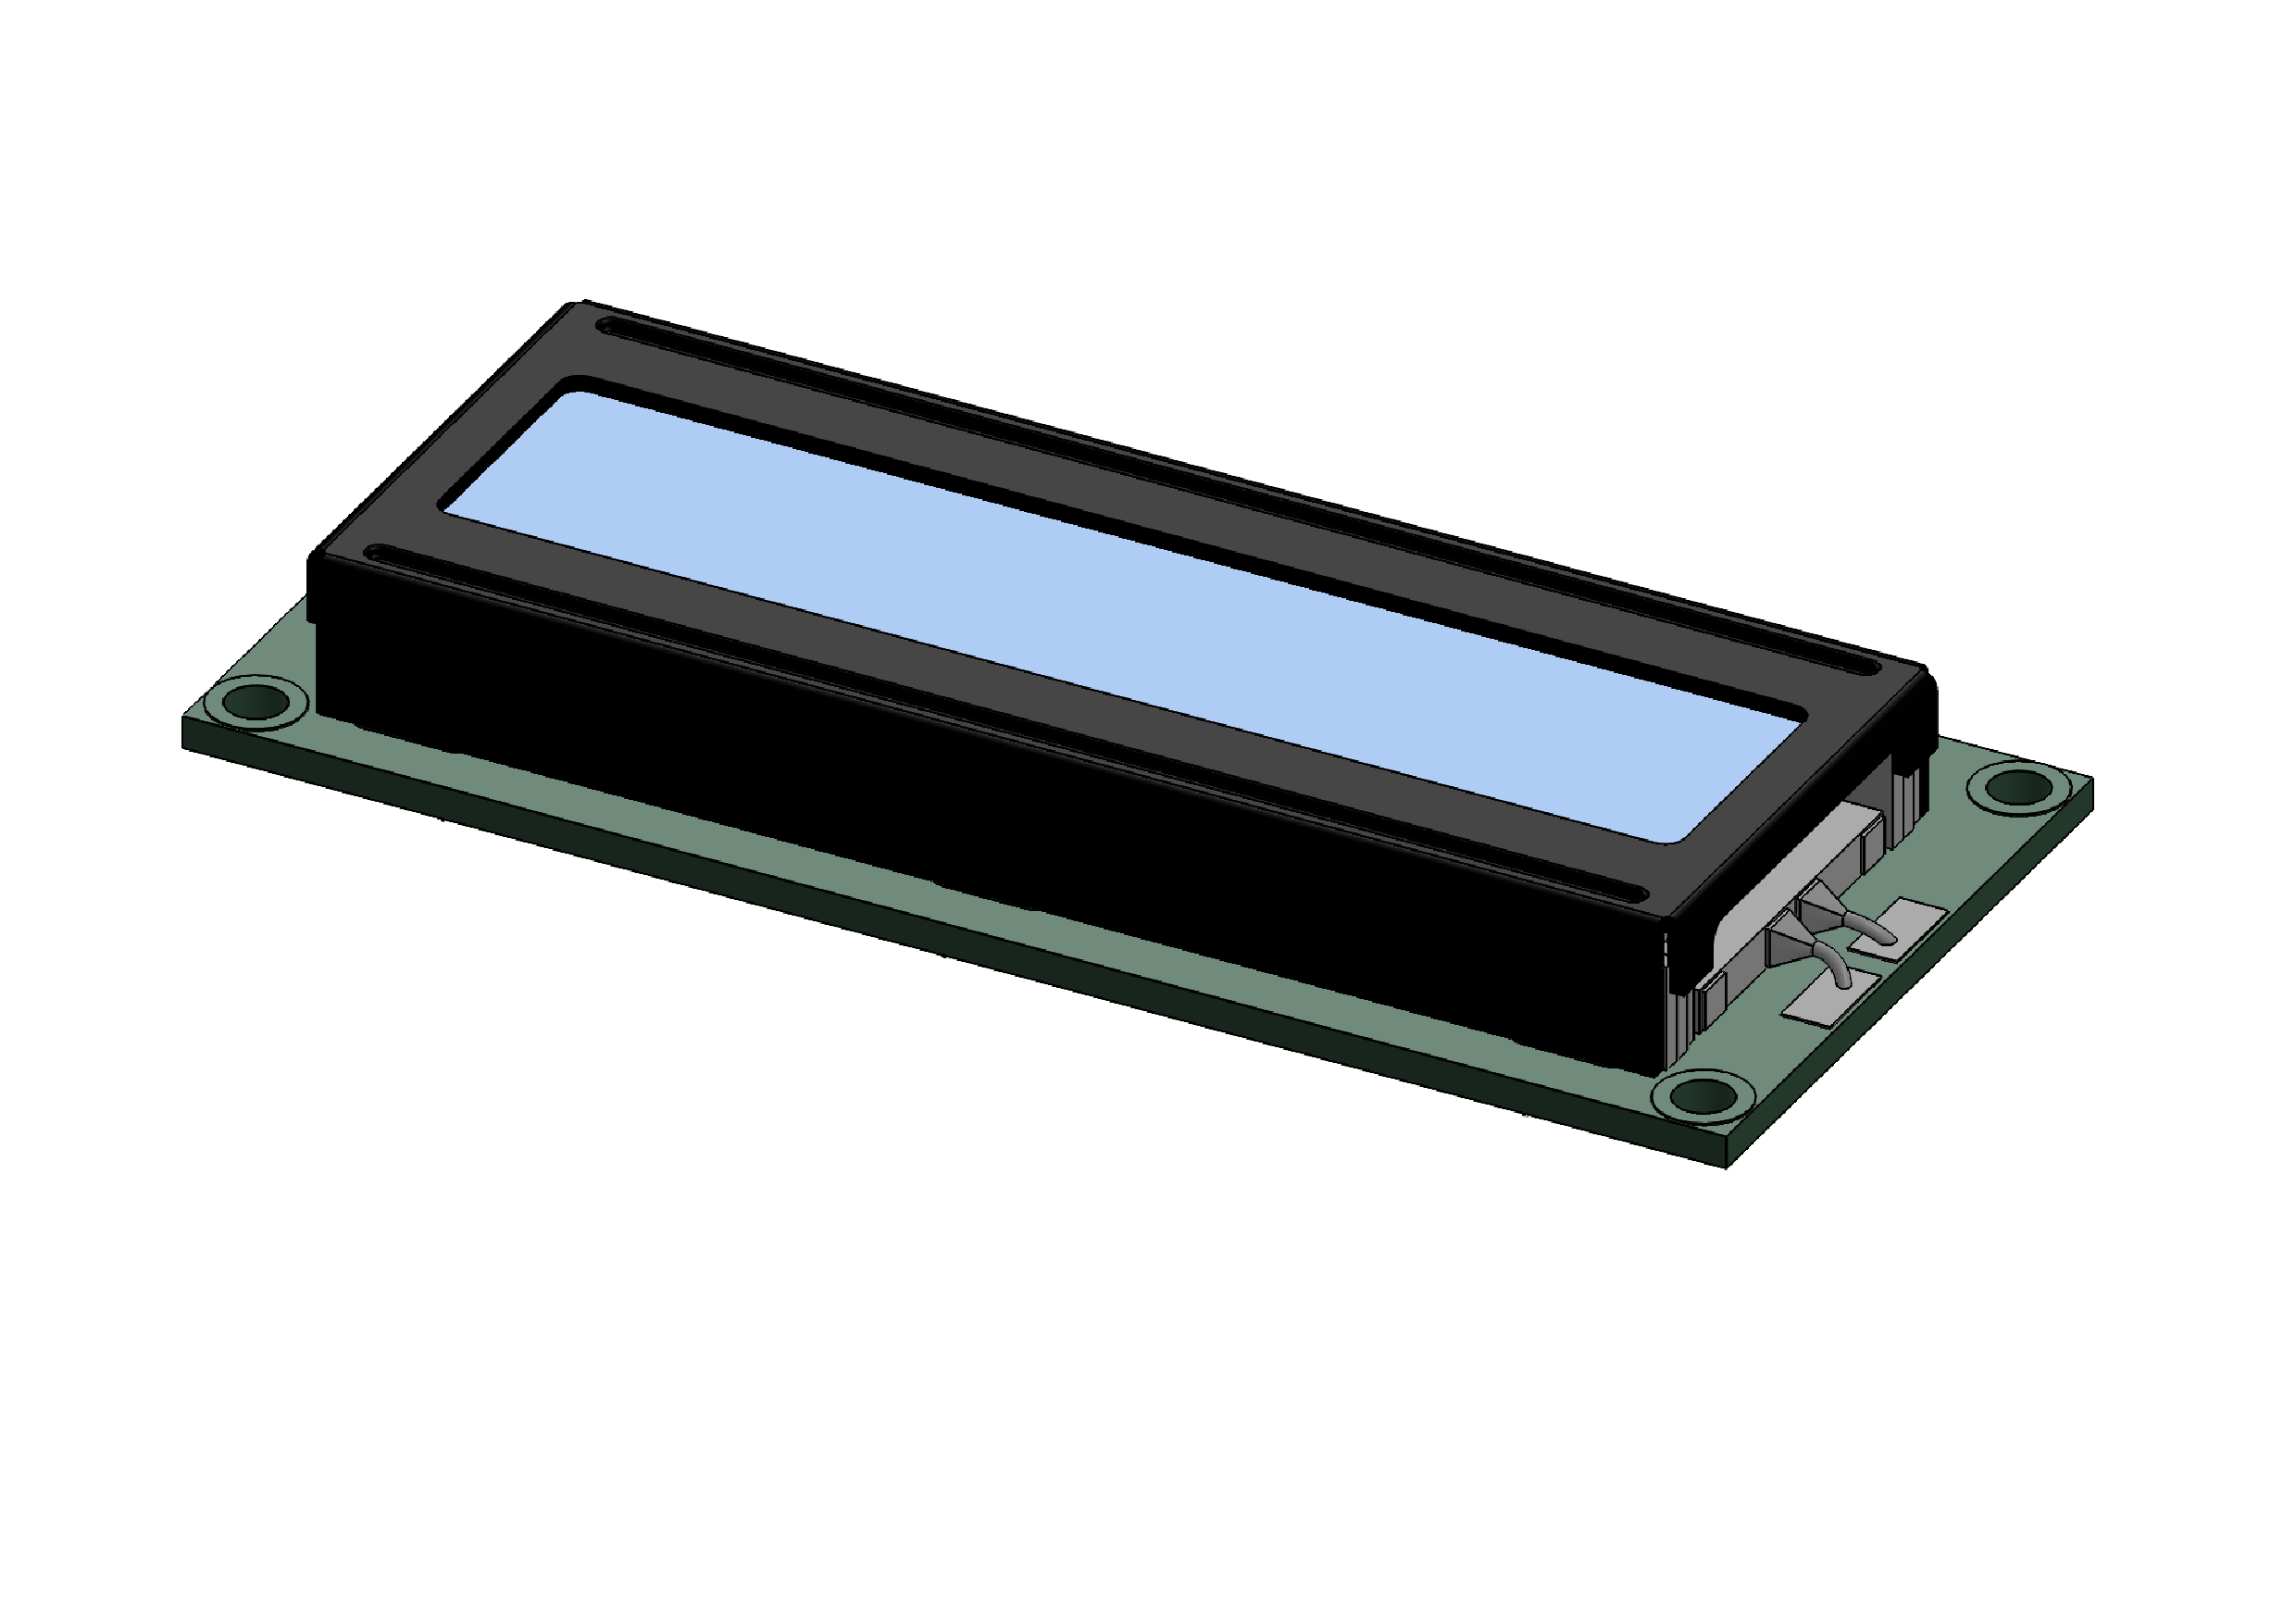
\includegraphics[height=19mm]{1/img/Pantalla Led.pdf}  & 
       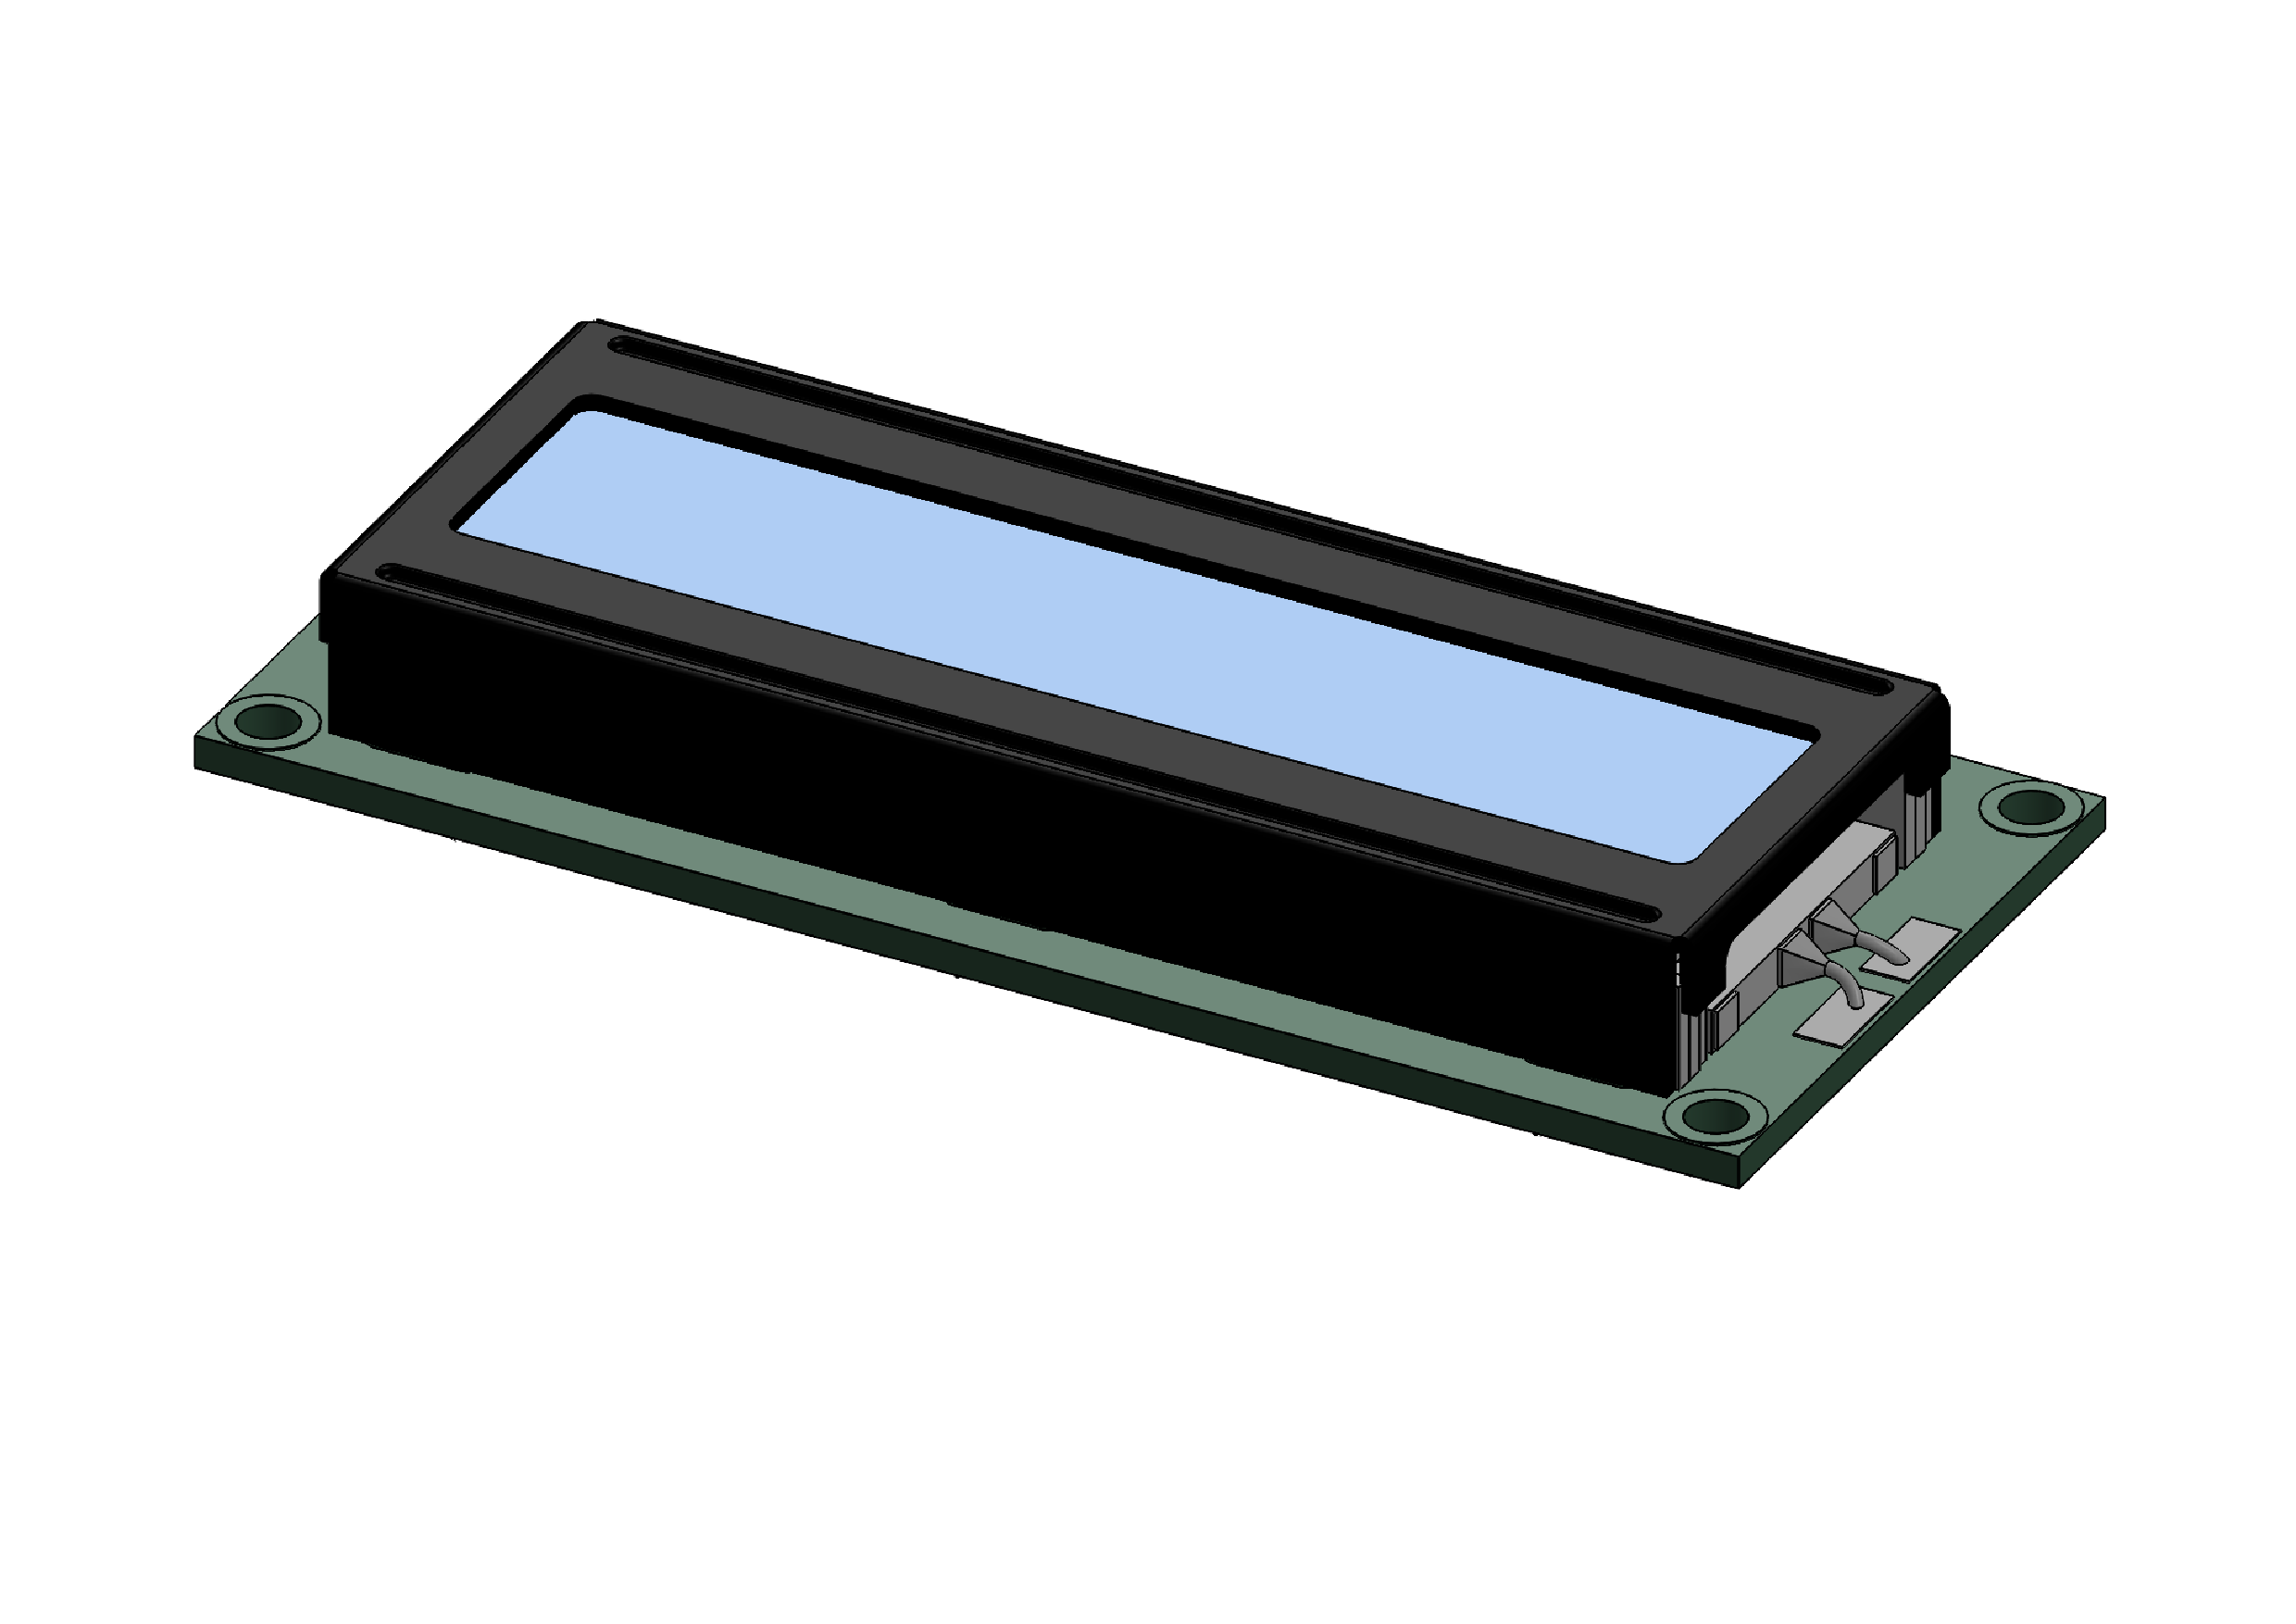
\includegraphics[width=19mm]{1/img/Pantalla Led_1.pdf} \\
        \hline
       Potenciometro & 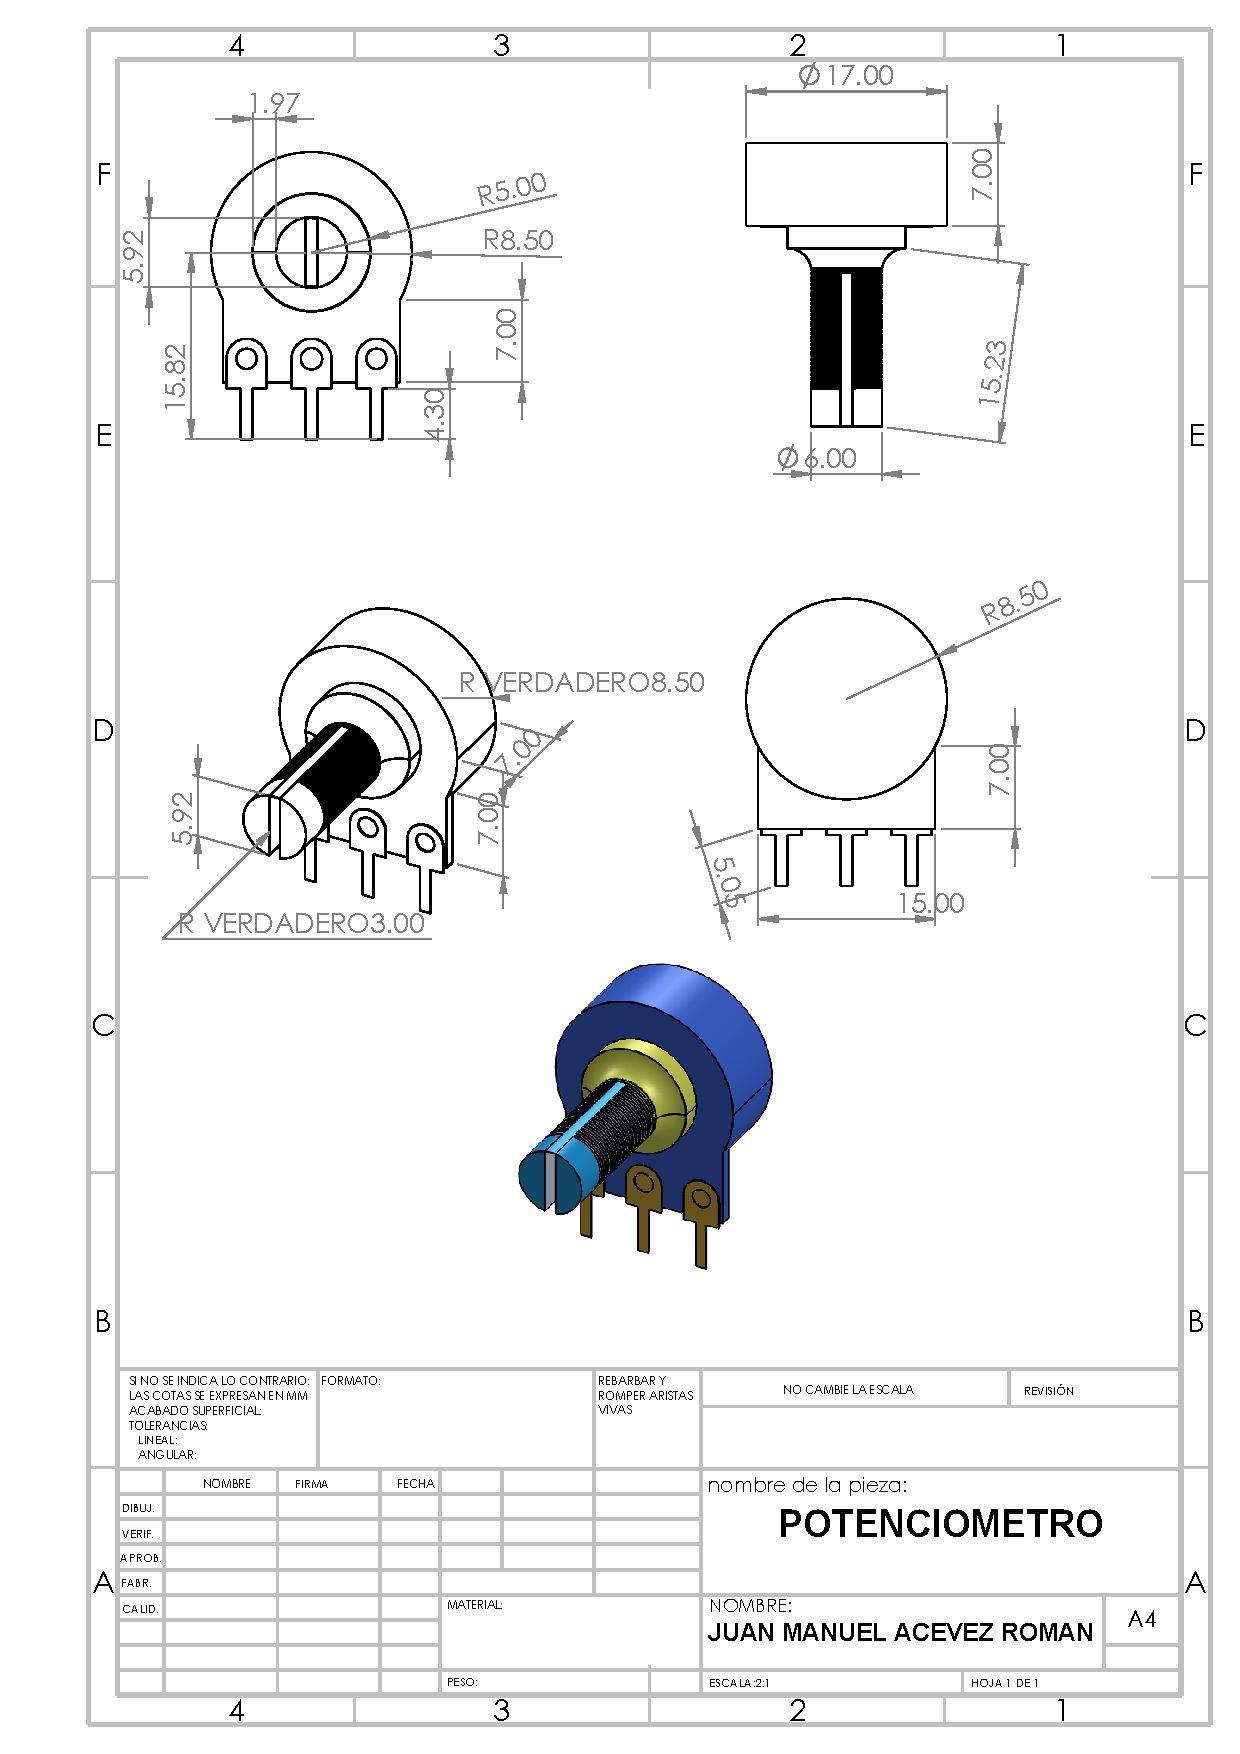
\includegraphics[height=19mm]{1/img/Potenciometro.pdf}  & 
       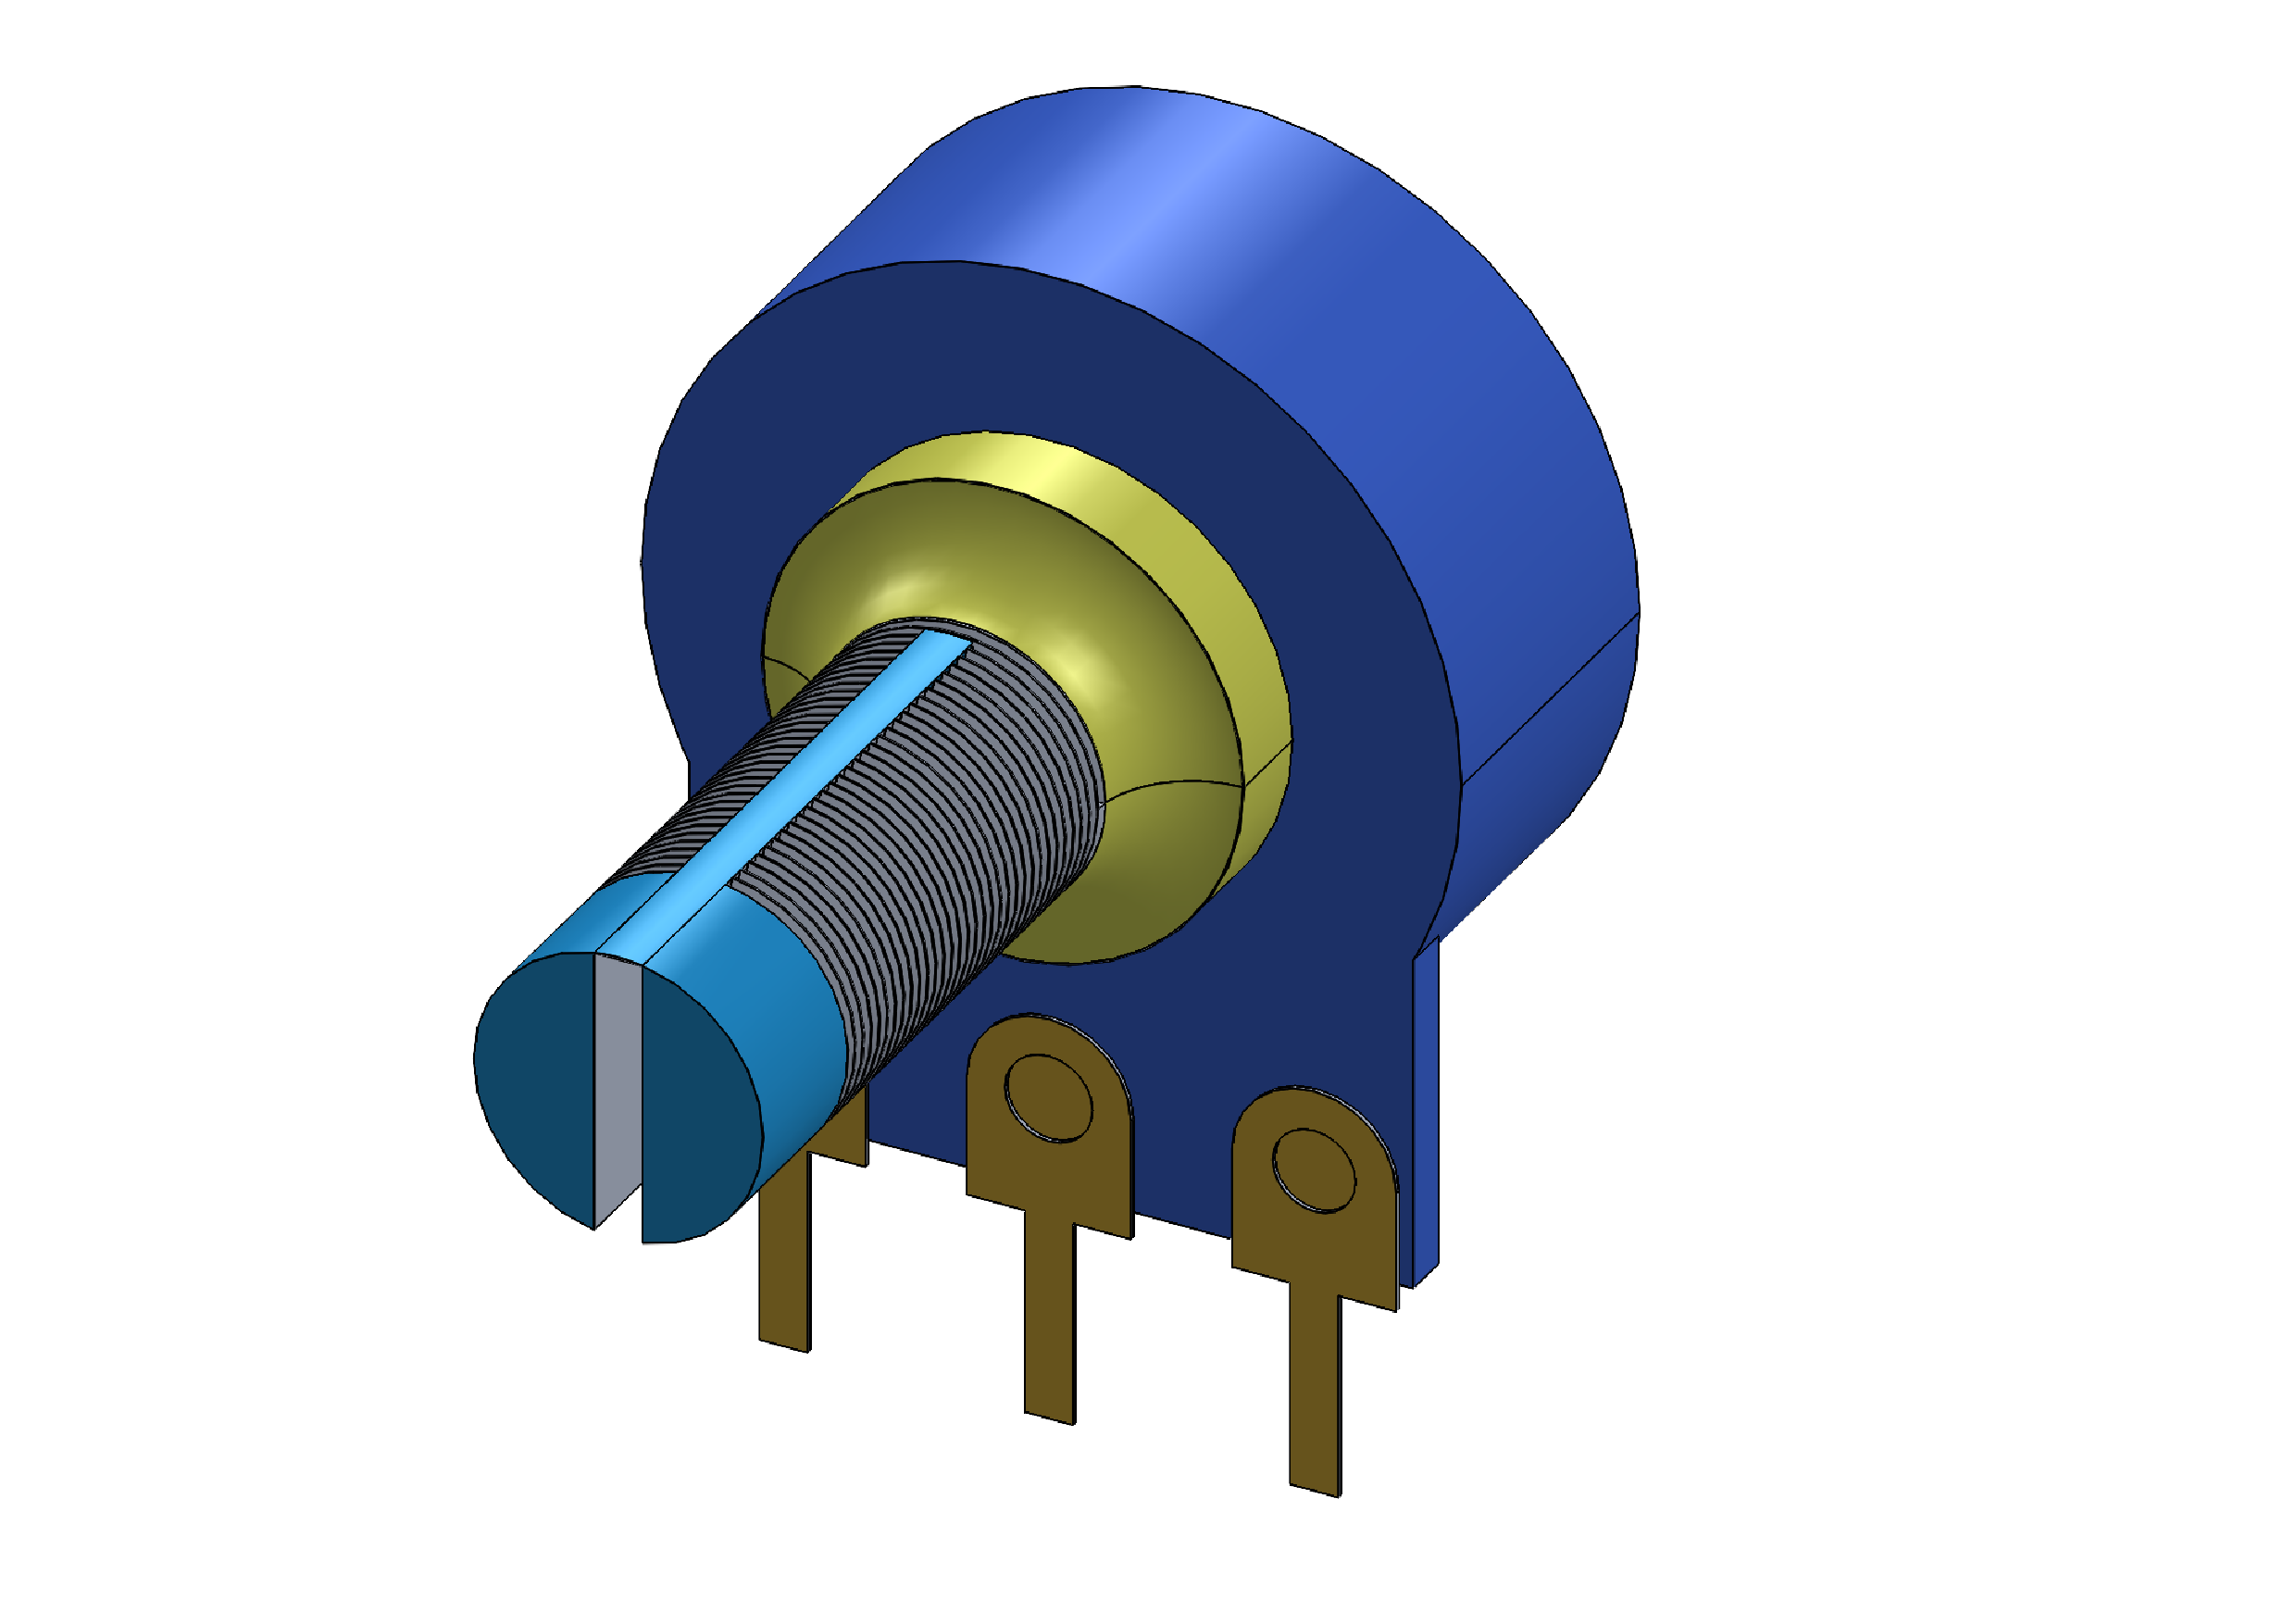
\includegraphics[width=19mm]{1/img/Potenciometro_1.pdf} \\
        \hline
       
        Resistencia & 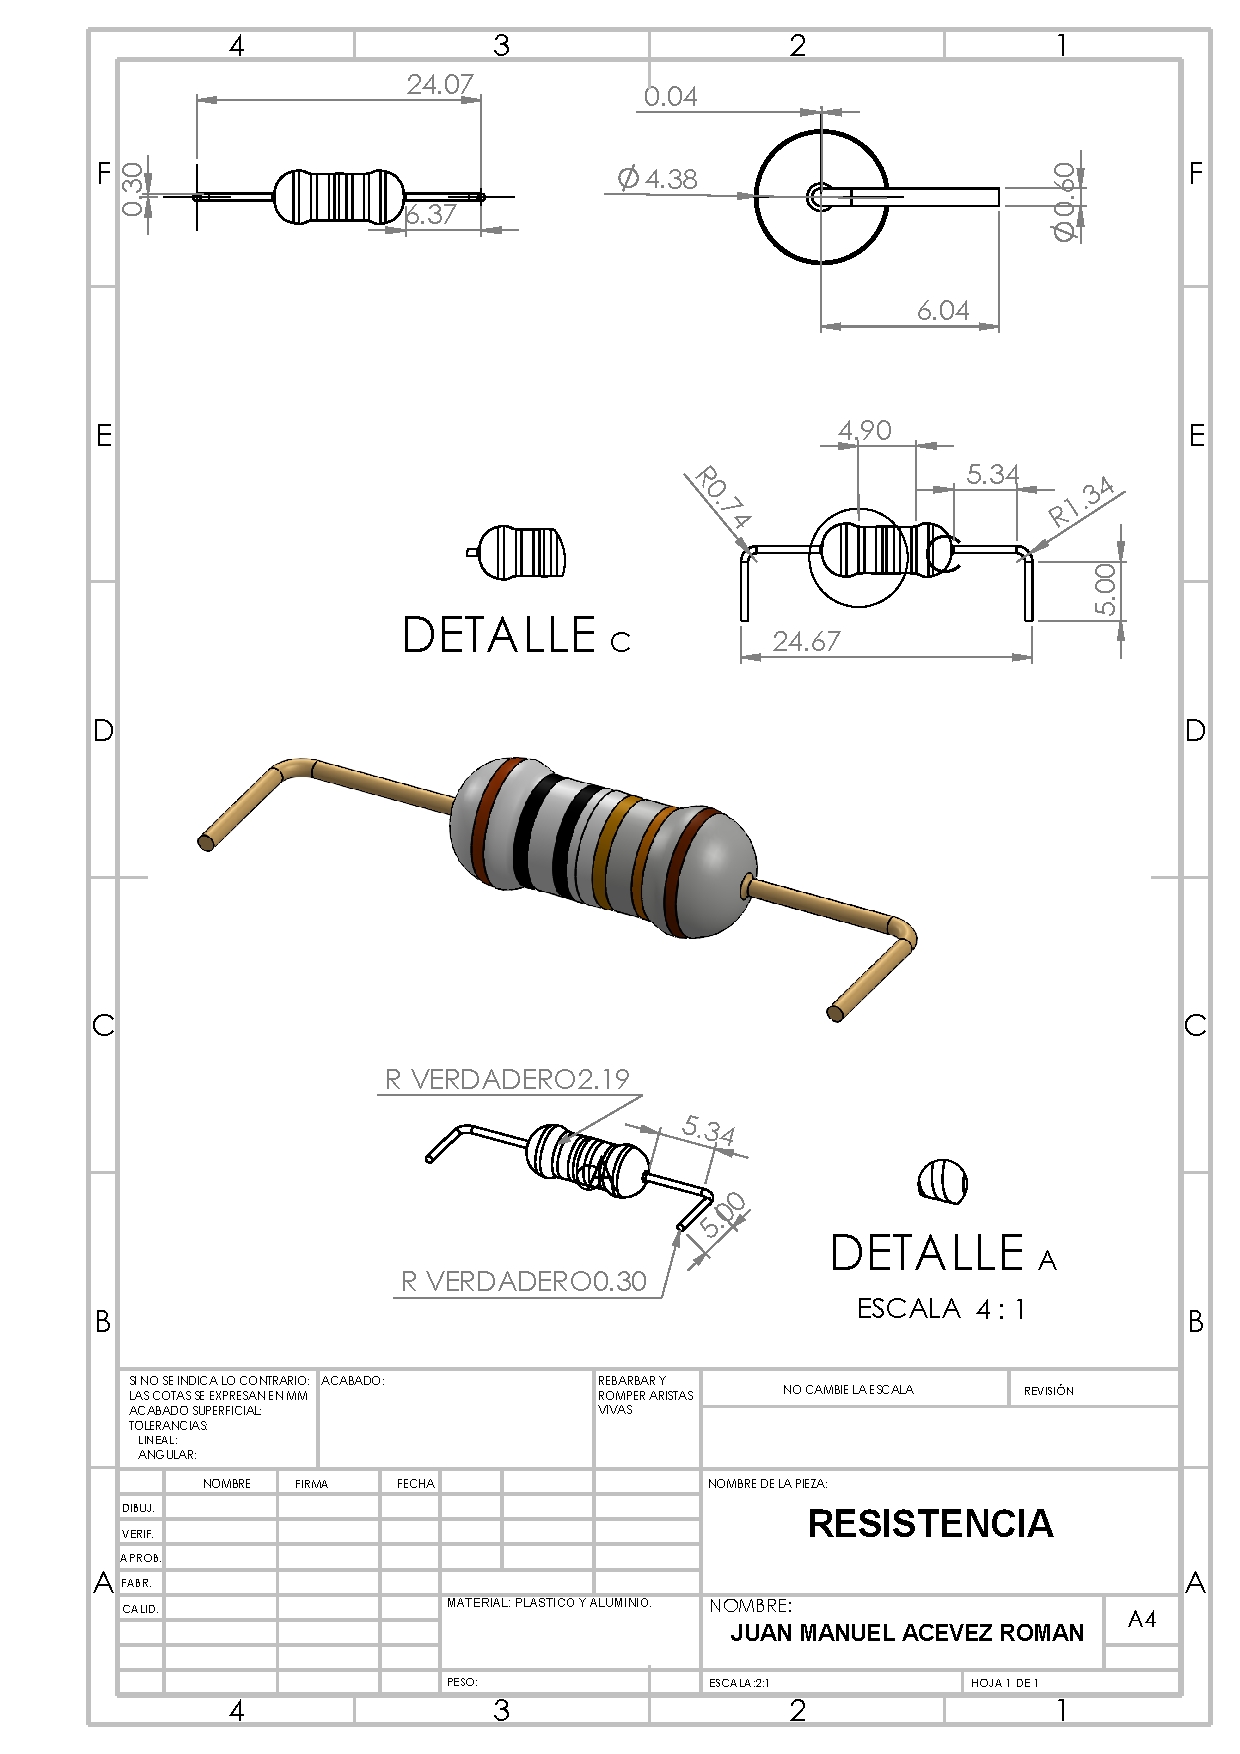
\includegraphics[height=19mm]{1/img/Resistencia.pdf}  & 
       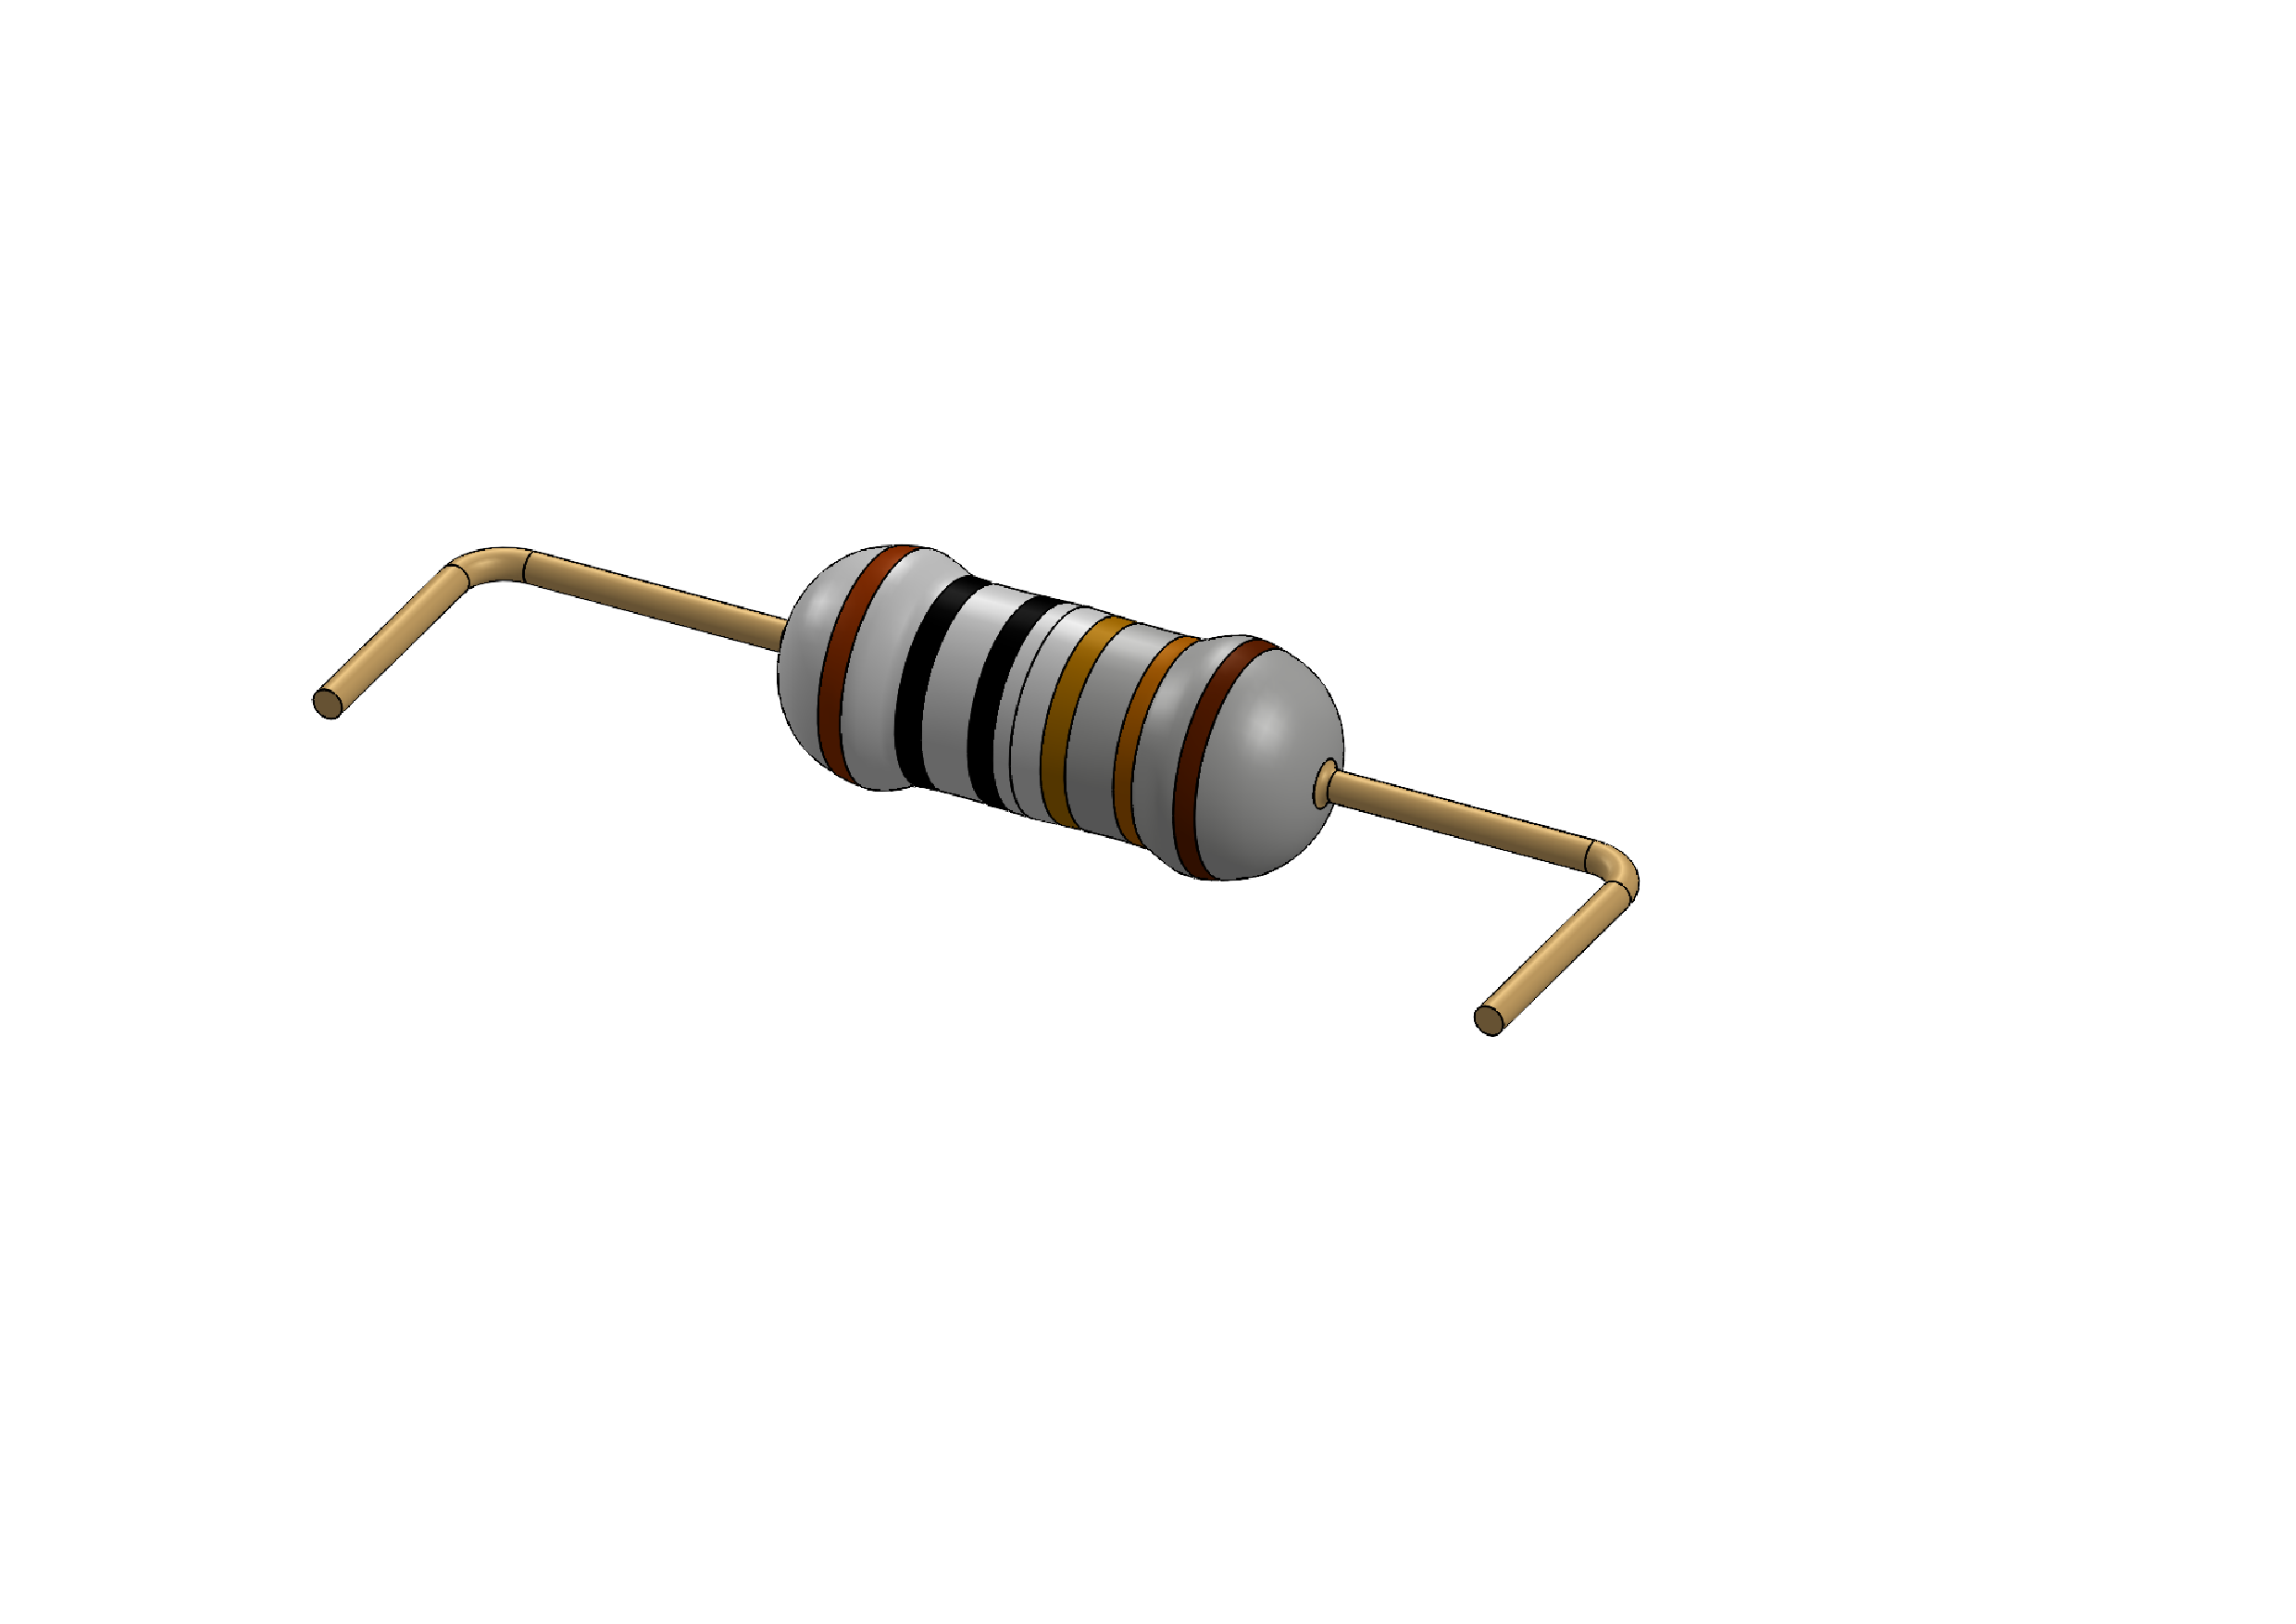
\includegraphics[width=19mm]{1/img/Resistencia_1.pdf} \\
        \hline 
       
        
        \end{tabular} 
       
         \label {tab : my_label}  \label {}
          \end{table} 
    
      \begin{tabular}{c|c}
           &  \\
           & 
      \end{tabular}
    
        
    \begin{itemize}
        
    \item \textbf{Identificación de Componentes y Herramientas:}
    %Analizar diagramas y especificaciones técnicas.
    %Elaborar una lista detallada de materiales y herramientas necesarias.
    
    \item \textbf{Establecimiento de Procedimientos de Ensamblaje:}
    %Desarrollar un proceso paso a paso para el ensamblaje.
    %Validar el procedimiento mediante pruebas piloto.
    
    \item \textbf{Definición de Tiempos y Movimientos:}
    %Cronometrar y analizar cada paso del proceso.
    %Optimizar movimientos y tiempos para mejorar la eficiencia.
    
    \item \textbf{Desarrollo de Protocolos de Prueba:}
    %Establecer criterios de prueba y procedimientos.
    %Documentar los resultados de las pruebas realizadas.
        
    \end{itemize}
    % 
    % 
    \begin{figure}[H]
        \centering
        \includegraphics[trim = {30mm 65mm 90mm 250mm},clip,scale=0.5]{1/img/IMG_4856.JPG}
        \caption{Esquema LCD de 16x2}
        \label{fig:IMG_4856.JPG}
    \end{figure}
    % 
    % 
    \begin{figure}[H] 
        \centering
        \includegraphics[trim = {30mm 250mm 90mm 20mm},clip,scale=0.5]{1/img/ESP-32.jpg}
        \caption{Esquema LCD de 16x2}
    
    
        \label{fig:img/ESP-32.jpg}
    \end{figure}
    % 
    % 
    \subsection{Prepara tu documento}
    
    Antes de que comiences a utilizar esta plantilla, es recomendable que prepare la información que contendrá en un archivo aparte. 
    Ten preparadas tus gráficas, así como también las tablas aparte, para que sea más fácil integrarlo. 
    Se recomienda fuertemente el uso de \textbf{formato Enhanced Metafile (.emf) para imágenes y gráficas} de resolución óptima. 
    Finalmente, completa y organiza el contenido antes de darle el formato de esta plantilla. 
    
    \subsection{Acrónimos y Abreviaciones}
    
    Los acrónimos y abreviaciones deberán ser definidos únicamente la primera vez que aparecen en el texto, esto para que el lector entienda lo que significan.
    
    \subsection{Ecuaciones}
    
    Las ecuaciones son una excepción a las especificaciones prescritas de esta plantilla. 
    Deberá determinar si su ecuación debe escribirse o no utilizando la fuente Adobe Devangari. 
    Para crear ecuaciones multinivel, puede ser necesario tratar la ecuación como un gráfico e insertarla en el texto después de aplicar el estilo de la platilla.
    Las ecuaciones serán enumeradas de manera consecutiva, y el número de ecuación, entre paréntesis, se colocan al ras de la derecha, utilizando una tabulación derecha. 
    
    \begin{equation}
        \label{eq1}
        x + y = z 
    \end{equation}
    
    Es importante asegurarse de que los símbolos de la ecuación sean definidos antes o inmediatamente después de la ecuación. Utilice “(1)”, en vez de “Eq. 1” al enumerar las ecuaciones, excepto al principio de una oración: “La ecuación (\ref{eq1}) es…”
    
    \section{Resultados y discusión}
    
    Antes de comenzar a preparar tu artículo, es importante que lea primero la guía del autor, la cual incluye los temas o apartados que son necesarios para tener tu trabajo completo.
    Una vez completada la edición del texto, el documento está listo para el uso de esta plantilla. En este archivo recién creado, resalte todo el contenido e importe el archivo de texto preparado. Ahora esta listo para estilizar su documento.
    En esta sección se deben presentar todo lo obtenido de la sección 2, incluidas deducciones o efectos del desarrollo. También se podrán incluir subsecciones numeradas de la siguiente forma:
    
    \subsection{Autores y Afiliaciones}
    
    Para distinguir las afiliaciones de los autores, utilice superíndices iniciando con el número 1, 2, etc., sucesivamente, esto dependerá de la cantidad de los departamentos a los que estén afiliados los autores. En caso de que todos los autores pertenezcan a una mismo departamento e institución, utilizar sólo el superíndice 1. 
    
    \subsection{Identificar los encabezados}
    
    Se les recuerda a los autores que los encabezados deben de estar conforme los solicita la guía del autor. De ahí se puede adaptar el trabajo para que sea más fácil de entender para el lector.
    Los encabezados organizan los temas sobre una base relacional y jerárquica. Por ejemplo, el título del documento es encabezado del texto principal porque todo el material posterior se relaciona y elabora sobre este tema. 
    
    \subsection{Tablas y Figuras}
    
    \begin{enumerate}
        \item Posición de las tablas y figuras: Coloque las figuras y las tablas en la parte superior e inferior de las columnas. Evite colocarlos en medio. Las figuras y las tablas grandes pueden abarcar ambas columnas. Los títulos de las figuras deben de estar debajo de las mismas; los títulos de las tablas deben aparecer encima de ellas. Insértese las figuras y los cuadros después de citarse en el texto. Utilice la abreviatura “Fig. 1”, incluso al principio de una oración. 
    \end{enumerate}
    
    \section{Conclusiones}
    
    Se describe aquí el alcance del trabajo, logros obtenidos y perspectivas para el futuro de este. Se sugiere colocar información cuantitativa obtenida.
    
    \section{Agradecimientos}
    
    Es importante darles su debido reconocimiento a los laboratorios, instituciones, organizaciones, entre otros que han sido participes para la culminación de este trabajo. También es importante mencionar, fondos, proyectos, becas, entre otros que se le han otorgado al o los autores para realizar el trabajo de investigación. Ejemplo: “Los autores agradecen al Concejo Nacional de Ciencia y Tecnología por los recursos otorgados…”
    
    \section*{Referencias}
    
    Para esta platilla, se solicita al autor enumerar las citas de manera consecutiva entre corchetes \cite{YLi2013}. 
    La puntuación de la oración que sigues sería \cite{Mesaelides2011}. 
    Refiérase simplemente al número de referencia, como en \cite{Morales2012}, no utilice “Ref. [3]” o “referencia [3]” excepto al principio de una oración: “La referencia [3] fue la primera…”
    Enumere las notas al pie por separado en superíndices. Coloque la nota de pie de en la parte inferior de la columna en la que se citó. No coloque notas al pie en la lista de referencias. Utilice letras para las notas al pie de la tabla.
    A menos de que haya tres autores o más; no utilice “et al.”. Los trabajos que no hayan sido publicados, incluso si han sido presentados para su publicación, deben ser citados como “inéditos”. Los trabajos que han sido aceptados para su publicación deben de citarse como “en prensa”. Poner en mayúscula sólo la primera palabra de un título, excepto los nombres propios y los símbolos de elemento. 
    Otros ejemplos \cite{LAAngeles2021}, \cite{LAAngelesConni}. 
    Véase el link \cite{prueba}.
    
    
    (1) \cite{Niebel}
    % Ejemplo
    %  @Article{article,
    % 	author = "Author1 LastName1 and Author2 LastName2 and Author3 LastName3",
    % 	title = "Article Title",
    % 	volume = "30",
    % 	number = "30",
    % 	pages = "10127-10134",
    % 	year = "2013",
    % 	doi = "10.3389/fnins.2013.12345",
    % 	URL = "http://www.frontiersin.org/Journal/10.3389/fnins.2013.12345/abstract",
    % 	journal = "Frontiers in Neuroscience"
    % }
    
    % @book{book,
    %   author    = {Author Name}, 
    %   title     = {The title of the work},
    %   publisher = {The name of the publisher},
    %   address   = {The city},
    %   year      = 1993,
    % }
    
    % @incollection{chapter,
    %   author       = {Bauthor Surname}, 
    %   title        = {The title of the work},
    %   editor       = {Editor Name},
    %   booktitle    = {The title of the book},
    %   publisher    = {The name of the publisher},
    %   address      = {The city},
    %   year         = 2002,
    %   pages        = {201-213},
    % }
    
    % @InProceedings{conference,
    %   author = {Cauthor Name and Dauthor Surname and Fauthor LastName},
    %   title = {The title of the work},
    %   booktitle = {The title of the conference proceedings},
    %   year = 1996,
    %   publisher = {The name of the publisher},
    %   editor = {Editor Name1 and Editor Name2},
    %   pages = {41-50},
    % }
    
    % @book{cho,
    %   author       = {Gauthor Name1}, 
    %   title        = {The title of the work},
    %   publisher = {Country code and patent number},
    %   address      = {Patent Country},
    %   year = 2013
    % }
    
    % @book{patent,
    %   author    = {Hauthor Surname1}, 
    %   title     = {The title of the work},
    %   publisher = {Patent number},
    %   address   = {Patent country},
    %   year      = 2010,
    % }
    
    % % please use misc for datasets
    % @misc{dataset, 
    % 	author = "Author1 LastName1 and Author2 LastName2 and Author3 LastName3",
    % 	title = "Data Title",
    % 	year = "2011",
    % 	doi = "10.000/55555",
    % 	URL = "http://www.frontiersin.org/",
    % }
    
    \bibliographystyle{ieeetr}
    \bibliography{1/referencias}
    % 
    % 
    %%%%%%%%%%%%%%%%%%%%%%%%%%%%%%%%%%
    \appendix
    %%%%%%%%%%%%%%%%%%%%%%%%%%%%%%%%%%
    % 
    % 
    \centering{\section[\appendixautorefname{}]{Apéndice}}\label{anexo:Manual de Ensamble}
    \includepdf[pages=-]{1/img/Manual de Ensamble.pdf}
    
    %%%%%%%%%%%%%%%%%%%%%%%%%%%%%%%%%%%%%%%%
    